\documentclass[a4paper, 11pt,UTF8]{ctexart}[draft]

%%%%%% 导入包 %%%%%%
\usepackage{CJKutf8}
\usepackage{graphicx}
\usepackage[unicode]{hyperref}
\usepackage{xcolor}
\usepackage{cite}
\usepackage{indentfirst}
\usepackage[fleqn]{amsmath}
\usepackage{amsthm}
\usepackage{amssymb}
\usepackage{fancyhdr}
\usepackage{color}
\usepackage{enumerate}
\usepackage{booktabs}
\usepackage[figuresright]{rotating}
\usepackage{overpic}
\usepackage{paralist}
\usepackage{mathrsfs}
\usepackage{multirow}
\usepackage{bbding}
\usepackage{pifont}
\usepackage{wasysym}
\usepackage{amssymb}
\usepackage{url}
\usepackage{hyperref}
\usepackage{colortbl}

\let\itemize\compactitem
\let\enditemize\endcompactitem
\let\enumerate\compactenum
\let\endenumerate\endcompactenum
\let\description\compactdesc
\let\enddescription\endcompactdesc

\allowdisplaybreaks[4] %允许公式跨页 1,2,3,4 4力度最大。



\renewcommand{\familydefault}{\ttdefault}  % 修改字体

%\rmdefault
%\sfdefault
%\ttdefault



\graphicspath{{ThesisFiles/}{Figure/}}

%%%%%% 代码环境自制%%%%%%
\usepackage{listings}
\usepackage{color}

\definecolor{dkgreen}{rgb}{0,0.6,0}
\definecolor{gray}{rgb}{0.5,0.5,0.5}
\definecolor{mauve}{rgb}{0.58,0,0.82}

\lstset{frame=shadowbox,
  language=c,
  aboveskip=3mm,
  belowskip=3mm,
  showstringspaces=false,
  columns=flexible,
  basicstyle={\small\ttfamily},
  numbers=none,
  numberstyle=\tiny\color{gray},
  keywordstyle=\color{blue},
  commentstyle=\color{dkgreen},
  stringstyle=\color{mauve},
  breaklines=true,
  breakatwhitespace=true,
  tabsize=3
}


\pagestyle{plain}%无页眉页脚



%%%%%% 设置字号 %%%%%%
\newcommand{\chuhao}{\fontsize{42pt}{\baselineskip}\selectfont}
\newcommand{\xiaochuhao}{\fontsize{36pt}{\baselineskip}\selectfont}
\newcommand{\yihao}{\fontsize{28pt}{\baselineskip}\selectfont}
\newcommand{\erhao}{\fontsize{21pt}{\baselineskip}\selectfont}
\newcommand{\xiaoerhao}{\fontsize{18pt}{\baselineskip}\selectfont}
\newcommand{\sanhao}{\fontsize{15.75pt}{\baselineskip}\selectfont}
\newcommand{\sihao}{\fontsize{14pt}{\baselineskip}\selectfont}
\newcommand{\xiaosihao}{\fontsize{12pt}{\baselineskip}\selectfont}
\newcommand{\wuhao}{\fontsize{10.5pt}{\baselineskip}\selectfont}
\newcommand{\xiaowuhao}{\fontsize{9pt}{\baselineskip}\selectfont}
\newcommand{\liuhao}{\fontsize{7.875pt}{\baselineskip}\selectfont}
\newcommand{\qihao}{\fontsize{5.25pt}{\baselineskip}\selectfont}

%%%% 设置 section 属性 %%%%
\makeatletter
\renewcommand\section{\@startsection{section}{1}{\z@}%
{-1.5ex \@plus -.5ex \@minus -.2ex}%
{.5ex \@plus .1ex}%
{\normalfont\sihao\CJKfamily{hei}}}
\makeatother

%%%% 设置 subsection 属性 %%%%
\makeatletter
\renewcommand\subsection{\@startsection{subsection}{1}{\z@}%
{-1.25ex \@plus -.5ex \@minus -.2ex}%
{.4ex \@plus .1ex}%
{\normalfont\xiaosihao\CJKfamily{hei}}}
\makeatother

%%%% 设置 subsubsection 属性 %%%%
\makeatletter
\renewcommand\subsubsection{\@startsection{subsubsection}{1}{\z@}%
{-1ex \@plus -.5ex \@minus -.2ex}%
{.3ex \@plus .1ex}%
{\normalfont\xiaosihao\CJKfamily{hei}}}
\makeatother

%%%% 段落首行缩进两个字 %%%%
\makeatletter
\let\@afterindentfalse\@afterindenttrue
\@afterindenttrue
\makeatother
\setlength{\parindent}{2em}  %中文缩进两个汉字位


%%%% 下面的命令重定义页面边距,使其符合中文刊物习惯 %%%%
\addtolength{\topmargin}{-54pt}
\setlength{\oddsidemargin}{0.63cm}  % 3.17cm - 1 inch
\setlength{\evensidemargin}{\oddsidemargin}
\setlength{\textwidth}{14.66cm}
\setlength{\textheight}{24.00cm}    % 24.62

%%%% 下面的命令设置行间距与段落间距 %%%%
\linespread{1.4}
% \setlength{\parskip}{1ex}
\setlength{\parskip}{0.5\baselineskip}

%%%%公式编号章关联
\makeatletter
\@addtoreset{equation}{section}
\makeatother

%%%% 正文开始 %%%%
\begin{document}
\begin{CJK}{UTF8}{gbsn}

%%%% 定理类环境的定义 %%%%
\newtheorem{example}{例}             % 整体编号
\newtheorem{algorithm}{算法}
\newtheorem{theorem}{定理}[section]  % 按 section 编号
\newtheorem{definition}{定义}
\newtheorem{axiom}{公理}
\newtheorem{property}{性质}
\newtheorem{proposition}{命题}
\newtheorem{lemma}{引理}
\newtheorem{corollary}{推论}
\newtheorem{remark}{注解}
\newtheorem{condition}{条件}
\newtheorem{conclusion}{结论}
\newtheorem{assumption}{假设}

%%%% 重定义 %%%%
\renewcommand{\contentsname}{目录}  % 将Contents改为目录
\renewcommand{\abstractname}{摘要}  % 将Abstract改为摘要
\renewcommand{\refname}{参考文献}   % 将References改为参考文献
\renewcommand{\indexname}{索引}
\renewcommand{\figurename}{图}
\renewcommand{\tablename}{表}
\renewcommand{\appendixname}{附录}
\renewcommand{\algorithm}{算法}


%%%% 定义标题格式,包括title,author,affiliation,email等 %%%%
\title{ICTT}
\author{冯哲\footnote{电子邮件: 1194585271@qq.com}\\[2ex]
\xiaosihao 计算机科学与技术学院\\[2ex]
}
\date{\today}


%%%% 以下部分是正文 %%%%
\maketitle
\setcounter{tocdepth}{4}       %增加目录深度
\tableofcontents
\newpage



\section{命题时序逻辑}
\subsection{语法}
\noindent\textcircled{\footnotesize{1}}~notation: \\
   \indent Z:整数;\\
   \indent N:正整数;\\
   \indent $N_0$:非负整数;\\
   \indent Prop:可数原子命题;\\
   \indent operate:${^\lnot},\square,\bigcirc,\Diamond,;,\vee,\wedge,+,*$

\noindent\textcircled{\footnotesize{2}}~归纳定义命题公式:
\begin{equation}\nonumber
\begin{split}
&1.~~p\in Prop,p ~is ~a ~formula.\\
&2.~~p,q \in Prop,so ~are ~the ~constructs.\\
&~~~~~~~~~~p,q,p\wedge q,p;q,\bigcirc p,\square q,p^+,q^*.and~so~on.
\end{split}
\end{equation}

\subsection{语义}
\noindent\textcircled{\footnotesize{1}}~状态~S~,~B=\{true,false\}\\
\indent ~S~:~Prop~$\rightarrow$~B~~~~~~~~~~\{原子命题~$\rightarrow$~B\}\\
\indent ~状态是原子命题到真假集合的映射。

\noindent\textcircled{\footnotesize{2}}~区间\\
\indent 区间~$\sigma$~:~非空状态序列。\\
\indent 区间长度~:~~~有限区间~~~~~~finite~~~~$|\sigma|$~~,~~$|\sigma|=status-1$ \\
\indent~~~~~~~~~~~~~~~~~~~~~无限区间~~~~infinite~~~~w\\
\indent~~~~~~~~~~~~~~~~~~~~~统一{\color{red}{$\bigstar$}},~$N_w=N_0\vee\{w\}$

operator~~$=,<,\leq,\preceq$\\
\indent~~~~对于~~~~$N_w~~,~w=w$\\
\indent~~~~对于~$i\in N_0,~i<w$\\
\indent~~~~$\preceq~~as~~\leq~-\{{w,w}\}$\\
\indent定义:\\
\indent~~~~1.~$\sigma~as~<s_0,...,s_{|\sigma|}>$~,~若~$\sigma~is~infinite.~~s_{|\sigma|}$~无定义。\\
\indent~~~~2.~$\sigma_{(i,...j)}~as~(0\leq i\preceq ~\leq |\sigma|)~<s_i,...s_j>$\\
\indent~~~~3.~$\sigma^{(k)}~as~(0\leq k \preceq |\sigma|)~<s_k,...,s_{|\sigma|}>$\\


%\subsection{可满足性与有效性}
%\subsection{时序操作符}
%\subsection{操作符的优先规则}
%\subsection{等价关系}
%\subsection{逻辑法则}




%\newpage
%\section{一阶时序逻辑}
%\subsection{语法}
%\subsection{语义}
%\subsection{可满足性与有效性}
%\subsection{逻辑法则}
\newpage
\section{PTL练习题}

\noindent常用基本符号优先级:\\
$1.~~{^\lnot}$\\
$2.~\bigcirc,\Diamond,\square,+,*$\\
$3.~~\wedge,\vee$\\
$4.~\rightarrow,\leftrightarrow$\\
$5.~~;$

\textbf{2018/7/22}

\noindent题~1~:~存在原子命题A,B,将下列命题用PTL公式表示:\\
\textcircled{\footnotesize{1}}~~A发生,那么之后B总会发生(包括当前状态)。\\
\textcircled{\footnotesize{2}}~~A发生,那么之前B总会发生(包括当前状态)。\\
答:\\
\textcircled{\footnotesize{1}}~~$\square(A\rightarrow\Diamond B)$ \\
{\color{red}{\textcircled{\footnotesize{2}}~~$^\lnot(\square^\lnot B;A)$}\\
理解:chop 分为两个区间,两个区间上分别真假共四种情况,而此时否定一种,剩三种,与\textcircled{\footnotesize{1}}的蕴含效果一样,具体情况为$ ^\lnot(P;Q) $被这样的区间满足:对于该区间的任意一种两段划分,要么第一段不满足P,要么第二段不满足Q (可以 第一段不满足P 同时 第二段不满足Q)。}

\textbf{2018/7/23}

\noindent题~2~:~存在原子命题A,B,假设有个词语"严格之后"表示之后的状态,但不包括当前状态。
"严格之前"同理,将下列命题用PTL公式表示:\\
\textcircled{\footnotesize{1}}~~A发生,那么严格之后B总会发生(不包括当前状态)。\\
\textcircled{\footnotesize{2}}~~A发生,那么严格之前B总会发生(不包括当前状态)。\\
答:\\
\textcircled{\footnotesize{1}}~~$\square(A\rightarrow\bigcirc\Diamond B)$ \\
\textcircled{\footnotesize{2}}~~$^\lnot((\square(more\wedge{^\lnot B}));A)$~{\color{red}{$\times$}~~~~$~\square~$和~more连用表示无穷区间~}\\
\textcircled{\footnotesize{2}}~~$^\lnot((\square(\circleddash{^\lnot B}));A)$~{\color{red}{$\times$}~~~~$\circleddash$不能和always直接连用,因为第一个状态没有上一状态。}\\
\textcircled{\footnotesize{2}}~~$({^\lnot}A)\wedge((\Diamond B;\bigcirc A)\vee(\square{^\lnot A}))$~{\color{red}{?}}\\
\textcircled{\footnotesize{2}}~~$({^\lnot}A)\wedge{^\lnot(\square{^\lnot B;skip;A})}$~${\color{red}{\surd}}$~~~~{\color{red}{题目的隐含意思有A不可能发生在起始状态}}\\
\textcircled{\footnotesize{2}}~~$({^\lnot}A)\wedge{^\lnot(\square{^\lnot B;\bigcirc A})}$~${\color{red}{\surd}}$~~~~{\color{red}{题目的隐含意思有A不可能发生在起始状态}}\\

\newpage
\textbf{2018/7/25 ~Kun~整理笔记}
\begin{center}
\textbf{时序逻辑性质表达 }~~~~~-2018/5/21
\end{center}
是朋友才能发消息,如何表示?\\
是朋友:~f~;发消息:~s~。\\

\noindent\textcircled{\footnotesize{1}}~~经典逻辑表达:\\
a).~~~~$s\rightarrow f$~~~~~发消息必是朋友。\\
b).~${^\lnot} f\rightarrow {^\lnot}s$~~~不是朋友不能发消息\\
c).~${^\lnot} ( {^\lnot} f\wedge s )$~~~不是朋友且发消息是不对的~~(与b)等价)\\
d).~~~~$f\vee {^\lnot s}$~~~~~要么是朋友要么不发消息~~(与b),c)等价)\\



\noindent\textcircled{\footnotesize{2}}~~时序逻辑表示:\\
a).将来能发消息,现在一定是朋友。
$$\Diamond(\Diamond s \rightarrow f) ~weak~~~~~~~~~~\square(s\rightarrow f)$$
b).现在不是朋友,将来不能发消息。
$$\square({^\lnot} f \rightarrow{^\lnot} s)$$
c).现在不是朋友,将来能发消息是不对的。
$${^\lnot}\Diamond(\square{^\lnot}f;s)~~~~~~~~~~\square{^\lnot({^\lnot} f\wedge s)}$$
d).任何时刻,要么是朋友,要么不发消息。
$$\square(f\vee{^\lnot}s)$$
e).在是朋友之前不能发消息。
$$\Diamond(s\rightarrow\boxdot f)$$


\noindent Runtime~verification~for~LTL~and~TLTL ~:\\
$${^\lnot}s~until~f\equiv \square {^\lnot}s;skip;f$$

\part{paper}

\section{A decision procedure for propositional projection
temporal logic with infinite models}
\textbf{无限模型下命题投影时间逻辑(PPTL)的决策过程}

\begin{enumerate}[(1)]
  \item 无限模型下命题投影时间逻辑(PPTL)的可满足性;
  \item PPTL 公式的决策过程;
  \begin{enumerate}
    \item PPTL 的范式;
    \item PPTL 的范式图;
    \item 根据公式转换为范式;
    \item 构造给定公式的范式图;
  \end{enumerate}
  \item 扩展 PPTL 的决策过程;
\end{enumerate}

\noindent
\fbox{
\textbf{Question}~~\textcircled{\footnotesize{1}}~~~\textbf{ITL, PTL, PPTL?}
}\\
\noindent ITL(Interval Temporal Logic) 区间时序逻辑, 规范和验证并发系统。

\noindent PTL 投影时序逻辑,相对于 ITL 扩展了 无限模型和投影操作。

\noindent PPTL 命题投影时序逻辑。


\noindent\textcolor{red}{决策过程是为了检查 PPTL 公式的可满足性条件。}


\subsection{PPTL}
\subsubsection{语法}
$P : :=~p~|~\bigcirc ~P~| ~\neg ~P~\left|~P_{1}~ \vee ~P_{2}~\right|~\left(P_{1},~ \ldots,~ P_{m}~\right) ~prj ~P$

$\bigcirc$, \textcolor{red}{$prj$}, 基本的时间运算符。


\noindent
\fbox{
\textbf{Question}~~\textcircled{\footnotesize{2}}~~~\textbf{PPTL 的 投影操作?}
}\\
\subsubsection{语义}

\begin{enumerate}
  \item state(状态):\\
    命题公式到真假集的映射。$B=\{t ~r ~u~ e, ~f~ a ~l~ s ~e\}, ~s ~: ~\operatorname{Prop}~ \longrightarrow~ B$
  \item interval(区间):\\
    有限无限区间的统一定义;\\
    区间长度比较操作:$=,<, \leq, \preceq$
  \item interpretation(解释):\\
    三元组:$\mathcal{I}=(\sigma, ~k, ~j)$ \\
    $\sigma$, 区间。\\
    $k \preceq j \leq|\sigma|$

\end{enumerate}


\subsubsection{运算法则}

\begin{figure}[!h]
  \centering
  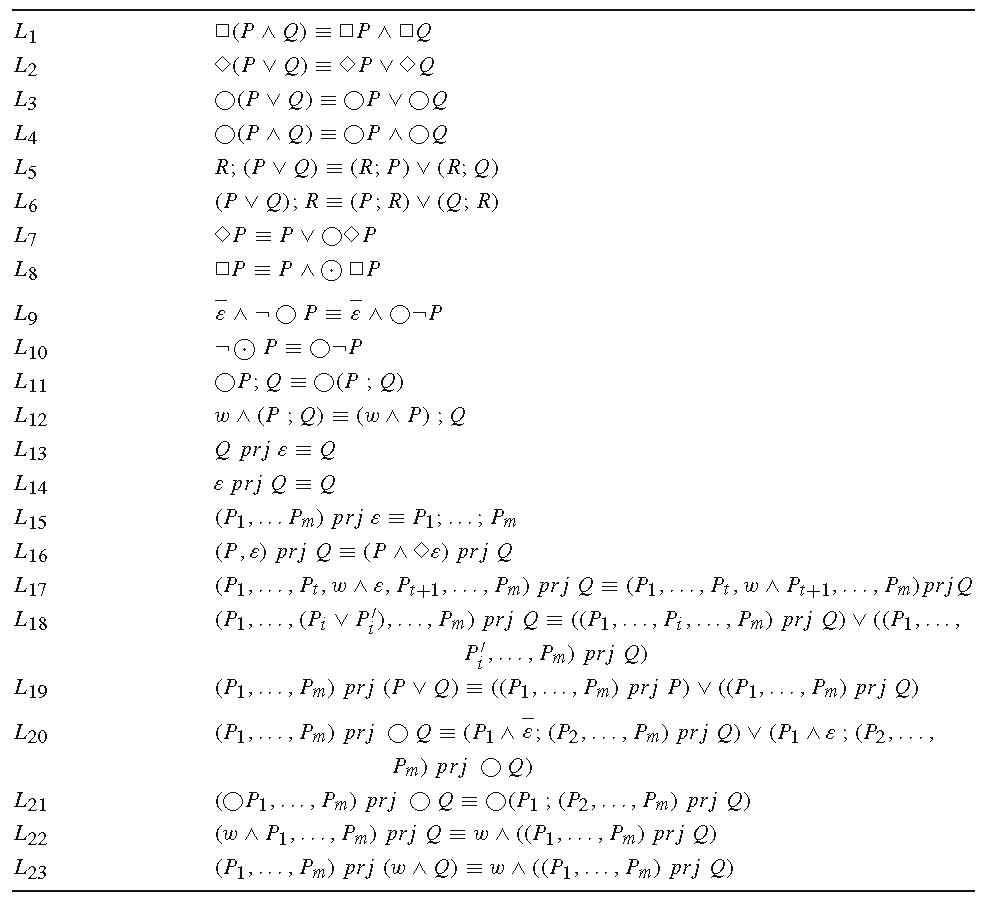
\includegraphics[width=1\textwidth]{law.png}
\end{figure}




\newpage
\part{Weekly conversation}
\section{2019/7/16}

\begin{enumerate}
  \item 范式:将 PPTL 公式化成规范形式。\\
  $$Q~\equiv~\bigvee_{j=1}^{n_{0}}\left(Q_{ej}~\wedge~\varepsilon\right)~\vee~\bigvee_{i=1}^{n}\left(Q_{ci}~\wedge~\bigcirc~Q_{i}^{\prime}\right)$$

  $Q$,PPTL范式;$Q_p$,原子命题公式;$Q_i^{\prime}$,普通 PPTL 公式。

  \noindent那么PPTL 公式怎么转为范式的四种情况:(最后一种为转为完全范式)。
  \begin{enumerate}[(1)]
    \item PPTL 公式转 $\mathrm{N}_{\mathrm{F}}$。
    \item project 操作转 $\mathrm{N}_{\mathrm{F}}$。
    \item chop 操作转 $\mathrm{N}_{\mathrm{F}}$。
    \item $\mathrm{N}_{\mathrm{F}}$ $\rightarrow$ $C\mathrm{N}_{\mathrm{F}}$\\
    例 $\mathrm{N}_{\mathrm{F}}$ 转 $C\mathrm{N}_{\mathrm{F}}$
    $$\begin{aligned}\left(p \wedge \bigcirc P^{\prime}\right) \vee\left(q \wedge \bigcirc Q^{\prime}\right) \equiv &\left((p \wedge q) \wedge \bigcirc\left(P^{\prime} \vee Q^{\prime}\right)\right) \vee\left((p \wedge \neg q) \wedge \bigcirc P^{\prime}\right) \\ & \vee\left((\neg p \wedge q) \wedge \bigcirc Q^{\prime}\right) \vee((\neg p \wedge \neg q) \wedge \bigcirc f a l s e) \end{aligned}$$

    $$\left(p \wedge \bigcirc P^{\prime}\right) \vee\left(q \wedge \bigcirc Q^{\prime}\right)=false \wedge  \epsilon \vee \left(p \wedge \bigcirc P^{\prime}\right) \vee\left(q \wedge \bigcirc Q^{\prime}\right)$$
  \end{enumerate}
  \item 完全范式(作用:PPTL 完全范式否定简易)

  $$Q~\equiv\left(Q_{e}~\wedge~\varepsilon\right)~\vee~V_{i=1}^{n}\left(Q_{i}~\wedge~\bigcirc~Q_{i}^{\prime}\right)$$

  其中 $\vee_{i}~Q_{i}~\equiv~\text~{~true~and~}~V_{i~\neq~j}\left(Q_{i}~\wedge~Q_{j}\right)~\equiv~false$。

  \item 完全范式的否定\\
  例 $C\mathrm{N}_{\mathrm{F}}$ 的否定
  $$\begin{aligned}\neg \big(\left(p \wedge \bigcirc P^{\prime}\right) \vee\left(q \wedge \bigcirc Q^{\prime}\right)\big) \equiv \neg \Big( &\left((p \wedge q) \wedge \bigcirc\left(P^{\prime} \vee Q^{\prime}\right)\right) \vee\left((p \wedge \neg q) \wedge \bigcirc P^{\prime}\right) \\ & \vee\left((\neg p \wedge q) \wedge \bigcirc Q^{\prime}\right) \vee((\neg p \wedge \neg q) \wedge \bigcirc f a l s e)\Big)\\ \equiv &\left((p \wedge q) \wedge \bigcirc\neg\left(P^{\prime} \vee Q^{\prime}\right)\right) \vee\left((p \wedge \neg q) \wedge \bigcirc\neg P^{\prime}\right) \\ & \vee\left((\neg p \wedge q) \wedge \bigcirc \neg Q^{\prime}\right) \vee((\neg p \wedge \neg q) \wedge \bigcirc\neg f a l s e) \end{aligned}$$

  \item 范式图(重点)\\
  \textcolor{red}{PPTL 公式决策过程的可视化}

  NFG 举例:
\begin{figure}[!h]
  \centering
  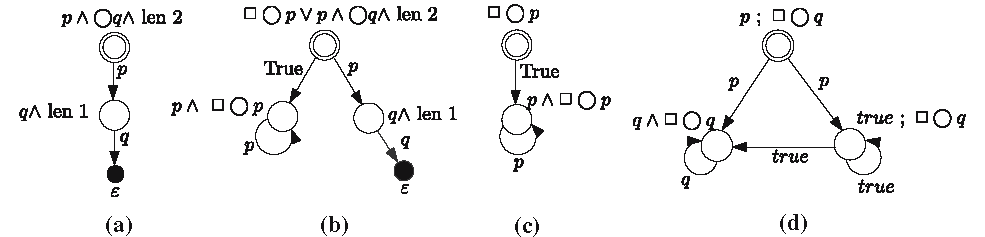
\includegraphics[width=1\textwidth]{NFG.png}
\end{figure}

  \item 带标签的范式图 \\
  由于 $prj$ 操作有明确的语义,$(P_1~,P_2)~prj~Q$ 的语义:
\begin{figure}[!h]
  \centering
  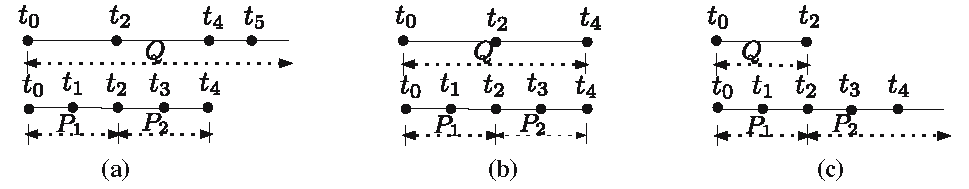
\includegraphics[width=1\textwidth]{prj.png}
\end{figure}

  即就是 PPTL 公式 $P_1$ 必须是有穷区间上的。但这一点在范式图上无法限制,所以加入标签。

\begin{figure}[!h]
  \centering
  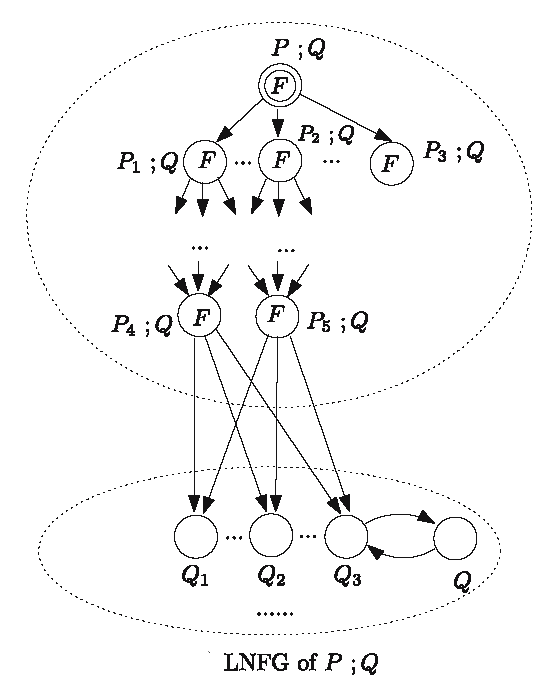
\includegraphics[width=0.6\textwidth]{LNFG.png}
\end{figure}
\end{enumerate}

\subsection{练习}

$\begin{array}{l}{\mathrm{NF}\left(\mathrm{O}^{2}(\square \bigcirc p ; q) \vee(p ; \square \bigcirc q)\right)} \\

\equiv \mathrm{NF}\left(\bigcirc^{2}(\square \bigcirc p ; q)\right) \vee \mathrm{NF}(p ; \square \bigcirc q) \\

\equiv \bigcirc(\bigcirc(\square \bigcirc p ; q)) \vee \operatorname{CHOP}(p ; \square \bigcirc q) \\

\equiv \bigcirc(\bigcirc(\square \bigcirc p ; q)) \vee \operatorname{CHOP}(\mathrm{NF}(p) ; \square \bigcirc q) \\

\equiv \bigcirc(\bigcirc(\square \bigcirc p ; q)) \vee \operatorname{CHOP}(p \wedge \varepsilon \vee p \wedge \text { Otrue; } \square \bigcirc q) \\

\equiv \bigcirc(\bigcirc(\square \bigcirc p ; q)) \vee \operatorname{CHOP}(p \wedge \varepsilon ; \square \bigcirc q) \vee \operatorname{CHOP}(p \wedge \text { Otrue; } \square \bigcirc q) \\

\equiv \bigcirc(\bigcirc(\square \bigcirc p ; q)) \vee p \wedge \operatorname{CHOP}(\varepsilon ; \square \bigcirc q) \vee p \wedge { \operatorname{CHOP}(\bigcirc true;} \square \bigcirc q ) \\

\equiv \bigcirc(\bigcirc(\square \bigcirc p ; q)) \vee p \wedge(\mathrm{NF}(\bigcirc q \wedge \varepsilon) \vee \mathrm{NF}(\bigcirc q \wedge \bigcirc \square \bigcirc q)) \vee p \wedge \bigcirc(\text {true} ; \square \bigcirc q) \\

{\equiv \bigcirc(\bigcirc(\square \bigcirc p ; q)) \vee p \wedge(f a l s e \vee \bigcirc(q \wedge \square \bigcirc q)) \vee p \wedge \bigcirc(\text {true} ; \square \bigcirc q)} \\ {\equiv \bigcirc(\bigcirc(\square \bigcirc p ; q)) \vee p \wedge \bigcirc(q \wedge \square \bigcirc q) \vee p \wedge \bigcirc(t r u e ; \square \bigcirc q)}
\end{array}$











\newpage



%
%\newpage
%
%\begin{table}[!h]
%\resizebox{\textwidth}{!}{
%\begin{tabular}{|l|l|l|l|l|}
%\hline
%价格                                                    & 备注          & 工期   & 物流(普通快递)   & 图片 \\ \hline
%8cm 12cm 共90张 纸片,塑胶硬套,通用绳 == 190元                     & 无           & 2-3天  & 3-4天  & 图一 \\ \hline
%8cm 12cm 厚度0.76mm(银行卡厚度) 共90张 PVC卡片带挂绳 3.5x90 == 315元 & 挂绳单面字印刷+50元 & 5天 & 3-4天 & 图二 (实图)\\ \hline
%8cm 12cm 厚度0.9mm (身份证厚度) 共90张 PVC卡片带挂绳 3.0x90 == 270元 & 挂绳印字+100元   & 刷绳3天 不刷绳1天  & 3-4天  & 图三(实图) \\ \hline
%8cm 12cm 厚度0.76mm 共90张 PVC卡片带挂绳 2.0x90 == 180元(推荐店家促销走量)    & 挂绳印字+95元    & 刷绳3天 不刷绳1天   & 3-4天 & 图四(实图) \\ \hline
%\end{tabular}}
%\end{table}
%
%\begin{figure}[!h]
%  \centering
%  \includegraphics[width=1.9in]{1.jpg}
%\end{figure}
%
%\begin{figure}[!h]
%  \centering
%  \includegraphics[width=1.9in]{2.jpg}
%\end{figure}
%
%\begin{figure}[!h]
%  \centering
%  \includegraphics[width=1.9in]{3.jpg}
%\end{figure}
%
%\begin{figure}[!h]
%  \centering
%  \includegraphics[width=1.9in]{4.jpg}
%\end{figure}
%
%
%\newpage
%胸牌设计:
%
%
%\noindent注:\\
%在明后两天确定设计图,工期上在下周基本可以拿到胸牌。

\newpage
\part{神经网络形式化}

\section{全连接神经网络}

\subsection{数学推导}

\subsubsection{作用过程示例}

%\begin{figure}[!h]
%  \centering
%  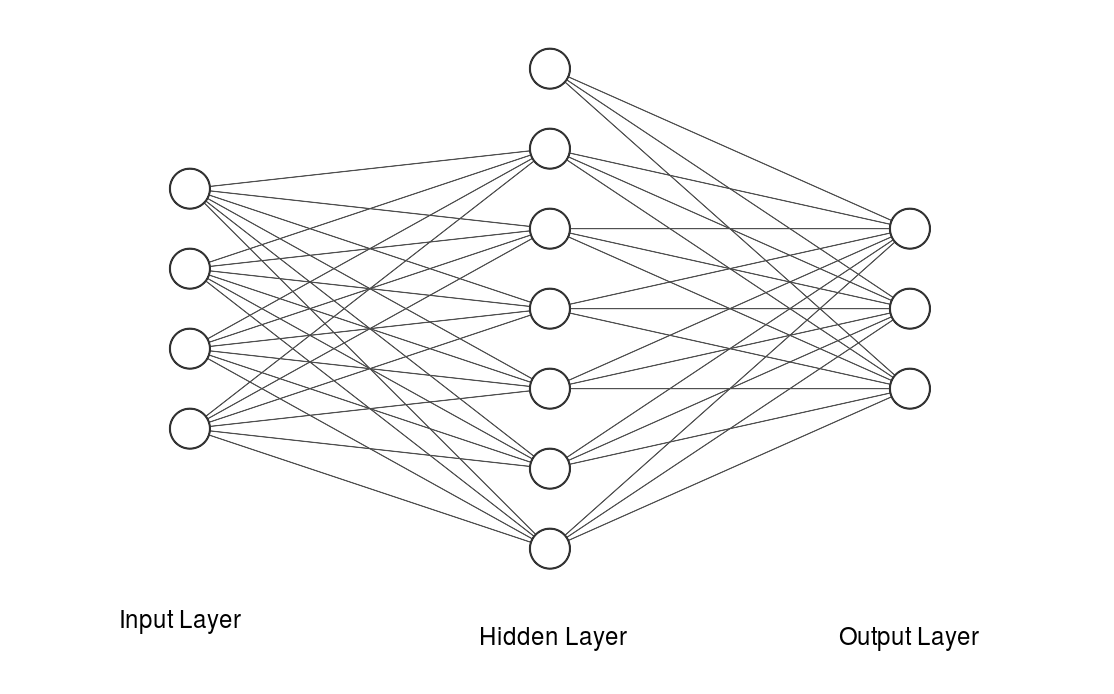
\includegraphics[width=1\textwidth]{FC.png}
%\end{figure}

\noindent\textcolor{red}{\textbf{变量说明:}}
\begin{itemize}
  \item 以零为下角标的变量为 偏置(bias)。
  \item $x$ 表示输入数据(一个训练样本为一个行向量),$y$ 表示标签(one-hot 编码,为一个行向量),$s$~为求和值,$a$~为激活值。
  \item $x^i_j$ 的上标表示第 i 行数据样本,下标表示该行数据样本的第 j 个值。
  \item $x,s,a$~若无下角标,则表示向量化。
  \item 多分类标签 $y$ 采用 one-hot 编码。
\end{itemize}

\begin{definition}
\textcolor{red}{向量上标+ 运算符}:为该向量添加Bias列,具体在第0列添加全1。\\
\textcolor{red}{~~~~~~~~~~~~~~~~向量上标- 运算符}:为该向量删去Bias列,具体删除第0列。
\end{definition}
\begin{example}
~~~~~~~$a = \left(
 \begin{matrix}
   a & b & c \\
   d & e & f \\
   g & h & i
  \end{matrix}
  \right) $~~~~~~
  $a^+ = \left(
\begin{matrix}
   1 & a & b & c \\
   1 & d & e & f \\
   1 & g & h & i
  \end{matrix}
  \right) $~~~~~~
  $a^- = \left(
\begin{matrix}
    b & c \\
    e & f \\
    h & i
  \end{matrix}
  \right) $
\end{example}
\begin{definition}
\textcolor{red}{同维矩阵对应位置相乘运算}:$A\circ B$ .
\end{definition}
\textbf{输入层三个神经元,一个隐藏层六个神经元,输出层三个神经元(三分类)为例。激活函数以逻辑函数,损失函数以均方差损失为例。}
~\\~\\


%\begin{overpic}[width=0.82\textwidth]{FC.png}
%
%    \put(12,45){\small $x_0^0$}
%
%    \put(15.3,44.8){\footnotesize$+1$}
%
%    \put(12,38){\small $x_1^0$}
%
%    \put(12,31){\small $x_2^0$}
%
%    \put(12,24){\small$x_3^0$}
%
%    \put(50,58){\small $a_0^1$}
%
%    \put(47.8,55.5){\footnotesize $+1$}
%
%    \put(47,51){\small $s_1^1|a_1^1$}
%
%    \put(47,44){\small $s_2^1|a_2^1$}
%
%    \put(47,37){\small$s_3^1|a_3^1$}
%
%    \put(47,30){\small $s_4^1|a_4^1$}
%
%    \put(47,23){\small $s_5^1|a_2^1$}
%
%    \put(47,16){\small $s_6^1|a_2^1$}
%
%    \put(84,41){\small$s_1^2|a_1^2$}
%
%    \put(84,34){\small $s_2^2|a_2^2$}
%
%    \put(84,27){\small $s_3^2|a_3^2$}
%
%    \put(30, 47){\small $w_{01}^1$}
%
%    \put(33, 44){\small $w_{11}^1$}
%
%    \put(37, 43){\small $w_{21}^1$}
%
%    \put(41, 43){\small $w_{31}^1$}
%
%    \put(64, 49){\small $w_{01}^2$}
%
%    \put(64, 45){\small $w_{11}^2$}
%
%    \put(64, 41.2){\small $w_{21}^2$}
%
%    \put(64, 37.4){\small $w_{31}^2$}
%
%    \put(64, 33.6){\small $w_{41}^2$}
%
%    \put(64, 29.8){\small $w_{51}^2$}
%
%    \put(64, 26){\small $w_{61}^2$}
%
%    \put(12, 18){\normalsize\bfseries $\big(\bm{x}^{(0)}\big)^+$}
%
%    \put(30, 12){\normalsize\bfseries {$ \bm{W_b}^{(1)}$}}
%
%    \put(42, 8){\normalsize\bfseries {$\bm{s}^{(1)}|\big(\bm{a}^{(1)}\big)^+$}}
%
%    \put(64, 13){\normalsize\bfseries {$\bm{W_b}^{(2)}$}}
%
%    \put(80, 18){\normalsize\bfseries $\bm{s}^{(2)}|\bm{a}^{(2)}$}
%
%    \put(8, 53){\normalsize Input Layer}
%    \put(40, 64){\normalsize Hidden Layer}
%    \put(76, 53){\normalsize Output Layer}
%
%\end{overpic}



\begin{overpic}[width=0.82\textwidth]{FC.png}

    \put(12,45){\scriptsize $x_0$}

    \put(15.7,44.8){\scriptsize$+1$}

    \put(12,38){\scriptsize $x_1$}

    \put(12,31){\scriptsize $x_2$}

    \put(12,24){\scriptsize$x_3$}

    \put(50.2,58){\scriptsize $a_0^{(1)}$}

    \put(47.9,55.5){\scriptsize $+1$}

    \put(47,51){\scriptsize $s_1^{(1)}|a_1^{(1)}$}

    \put(47,44){\scriptsize $s_2^{(1)}|a_2^{(1)}$}

    \put(47,37){\scriptsize$s_3^{(1)}|a_3^{(1)}$}

    \put(47,30){\scriptsize $s_4^{(1)}|a_4^{(1)}$}

    \put(47,23){\scriptsize $s_5^{(1)}|a_5^{(1)}$}

    \put(47,16){\scriptsize $s_6^{(1)}|a_6^{(1)}$}

    \put(84,41){\scriptsize$s_1^{(2)}|a_1^{(2)}$}

    \put(84,34){\scriptsize $s_2^{(2)}|a_2^{(2)}$}

    \put(84,27){\scriptsize $s_3^{(2)}|a_3^{(2)}$}

    \put(30, 47){\scriptsize $w_{01}^{(1)}$}

    \put(33, 44){\scriptsize $w_{11}^{(1)}$}

    \put(37, 43){\scriptsize $w_{21}^{(1)}$}

    \put(41, 43){\scriptsize $w_{31}^{(1)}$}

    \put(64, 49){\scriptsize $w_{01}^{(2)}$}

    \put(64, 45){\scriptsize $w_{11}^{(2)}$}

    \put(64, 41.2){\scriptsize $w_{21}^{(2)}$}

    \put(64, 37.4){\scriptsize $w_{31}^{(2)}$}

    \put(64, 33.6){\scriptsize $w_{41}^{(2)}$}

    \put(64, 29.8){\scriptsize $w_{51}^{(2)}$}

    \put(64, 26){\scriptsize $w_{61}^{(2)}$}

    \put(12, 18){\small $\bm{x}^+$}

    \put(30, 12){\small {$ \bm{W}^{(1)}$}}

    \put(42, 7){\small {$\bm{s}^{(1)}|\big(\bm{a}^{(1)}\big)^+$}}

    \put(64, 13){\small {$\bm{W}^{(2)}$}}

    \put(80, 18){\small $\bm{s}^{(2)}|\bm{a}^{(2)}$}

    \put(11, 53){\scriptsize\bfseries Input Layer}
    \put(43, 64){\scriptsize\bfseries Hidden Layer}
    \put(78, 53){\scriptsize\bfseries Output Layer}

\end{overpic}










\begin{overpic}[width=0.82\textwidth]{programExample3.png}
    %\put(82, 95.5){---}
    \put(82,90){ \tiny \uppercase\expandafter{\romannumeral1} }
    \put(81.5,64){ \tiny \uppercase\expandafter{\romannumeral2} }
    \put(81.1,40.3){ \tiny \uppercase\expandafter{\romannumeral3} }
    \put(81.5,36){ \tiny \uppercase\expandafter{\romannumeral4} }

    \put(75,18){\tiny \uppercase\expandafter{\romannumeral5}}

    \put(78.5,23){\tiny \uppercase\expandafter{\romannumeral6}}
    \put(77,10){\tiny \uppercase\expandafter{\romannumeral7}}

    \put(82.2,29){\tiny \uppercase\expandafter{\romannumeral8}}
\end{overpic}



\noindent\textbf{作用过程:}
\begin{enumerate}
  \item 向前传播计算误差:
  \begin{align*}
    & \big(x^{(0)}\big)^+w^{(1)}=s^{(1)},~~~\sigma(s^{(1)})=a^{(1)}\\
    & \big(a^{(1)}\big)^+w^{(2)}=s^{(2)},~~~\sigma(s^{(2)})=a^{(2)} \\
    & Loss~~~L=\frac{1}{2}\sum_{k=1}^{3}(a^{(2)}_k-y_k)^2
  \end{align*}

    \noindent假设有 1 个训练样本:
  \begin{enumerate}[(1)]
    \item $x$  的维度就是 $1\times 3$。
    \item $x^+$  的维度就是 $1\times 4$。
    \item $w^{(1)}$ 的维度就是 $4 \times 6$。
    \item $s^{(1)}$ 的维度就是 $1\times 6$。
    \item $a^{(1)}$ 的维度就是 $1 \times 6$。
    \item $\big(a^{(1)}\big)^+$ 的维度就是 $1 \times 7$。
    \item $w^{(2)}$ 的维度就是 $7 \times 3$。
    \item $s^{(2)}$ 的维度就是 $1\times 3$。
    \item $a^{(2)}$ 的维度就是 $1 \times 3$。 (输出层)
  \end{enumerate}
  \item 误差反向传播计算权值梯度:
  \begin{enumerate}[(1)]
    \item 输出层权值梯度:
      \begin{align*}
    Loss,~~~L&=\frac{1}{2}\sum_{i=1}^{K}(a^{(2)}_i-y_i)^2\\
    \frac{\partial L}{w^{(2)}_{ik}}&=\frac{\partial}{\partial w^{(2)}_{ik}}\frac{1}{2}\sum_{i=1}^{K}(a^{(2)}_i-y_i)^2\\
    &=\big(\sigma(s^{(2)}_k)-y_k\big)\sigma(s^{(2)}_k)\big(1-\sigma(s^{(2)}_k)\big)\frac{\partial s^{(2)}_k}{\partial w^{(2)}_{ik}}\\
    &=\big(\sigma(s^{(2)}_k)-y_k\big)\sigma(s^{(2)}_k)\big(1-\sigma(s^{(2)}_k)\big)\big(a^{(1)}_i\big)^+\\
    \text{令,}~~\delta^{(2)}_k&=\big(\sigma(s^{(2)}_k)-y_k\big)\sigma(s^{(2)}_k)\big(1-\sigma(s^{(2)}_k)\big)\\
    &=\big(a^{(2)}_k-y_k\big)a^{(2)}_k\big(1-a^{(2)}_k\big)\\
    \text{则,}\frac{\partial L}{w^{(2)}_{ik}}&=\delta^{(2)}_k\big(a^{(1)}_i\big)^+
  \end{align*}
    \item 隐藏层权值梯度:
    \begin{align*}
       \frac{\partial L}{\partial w^{(1)}_{ij}}&=\frac{\partial}{\partial w^{(1)}_{ij}}\frac{1}{2}\sum_{k\in K}(a^{(2)}_k-y_k)^2\\
       &=\sum_{k\in K}(a^{(2)}_k-y_k)\frac{\partial \sigma(s^{(2)}_k)}{\partial  w^{(1)}_{ij}}\\
       &=\sum_{k\in K}(a^{(2)}_k-y_k)\sigma(s^{(2)}_k)\big(1-\sigma(s^{(2)}_k)\frac{\partial s^{(2)}_k}{\partial  w^{(1)}_{ij}}\\
       &=\sum_{k\in K}(a^{(2)}_k-y_k)\sigma(s^{(2)}_k)\big(1-\sigma(s^{(2)}_k)\frac{\partial s^{(2)}_k}{\partial  a^{(1)}_{j}}\frac{\partial a^{(1)}_{j}}{\partial  w^{(1)}_{ij}}\\
       &=\sum_{k\in K}(a^{(2)}_k-y_k)\sigma(s^{(2)}_k)\big(1-\sigma(s^{(2)}_k)w^{(2)}_{jk}\frac{\partial a^{(1)}_{j}}{\partial  w^{(1)}_{ij}}\\
       &=\frac{\partial a^{(1)}_{j}}{\partial  w^{(1)}_{ij}}\sum_{k\in K}(a^{(2)}_k-y_k)\sigma(s^{(2)}_k)\big(1-\sigma(s^{(2)}_k)w^{(2)}_{jk}\\
       &=a^{(1)}_j\big(1-a^{(1)}_j\big)\frac{\partial s^{(1)}_j}{w^{(1)}_{ij}}\sum_{k\in K}\delta^{(2)}_kw^{(2)}_{jk}\\
       &=a^{(1)}_j\big(1-a^{(1)}_j\big)\big(x^{(0)}_i\big)^+\sum_{k\in K}\delta^{(2)}_kw^{(2)}_{jk}\\
       \text{令, }~~~ \delta^{(1)}_j &= a^{(1)}_j(1-a^{(1)}_j)\sum_{k \in K} \delta^{(2)}_kw^{(2)}_{jk}\\
       \text{则,} \frac{\partial L}{\partial w^{(1)}_{ij}}&= \delta^{(1)}_j \big(x_i^{(0)}\big)^+
    \end{align*}
  \end{enumerate}


  \item 更新权值:
  \begin{align*}
    W = W -\eta \frac{\partial Loss}{\partial W}
  \end{align*}
\end{enumerate}



\subsubsection{作用过程推广}

\noindent\textbf{用户指定神经网络相关参数:}
\begin{table}[!h]
\resizebox{\textwidth}{!}{
\begin{tabular}{|l|l|l|}
\hline
变量名称        & 符号    & 备注                                                                                                       \\ \hline\hline
训练样本维度      & $N_t$ &                                                                                                          \\ \hline
训练样本数量      & $N_T$ &                                                                                                          \\ \hline
隐藏层数       & $H$ & 包含H个隐藏层                                                                                                       \\ \hline
第i层神经元个数 & $N^{(i)}$ & \begin{tabular}[c]{@{}l@{}}$i=0,1,\cdots,H,H+1$\\$i=H+1$, 输出层,$N^i=K$\\ \textcolor{red}{这里定义不带 bias 神经元。}\end{tabular} \\ \hline

第i层的激活函数 & $\sigma^{(i)}$ & 在常用的 sigmoid,tanh,relu,leaky relu 中选择                                                                               \\ \hline
分类类别数       & K     &                                                                                                          \\ \hline
损失函数        & $S_l$ & 在常用的 MeanSquareError,CorssEntropyLoss 中选择                                                                \\ \hline
\end{tabular}}
\end{table}

~\\
\noindent\textbf{常见激活函数:}
\begin{enumerate}
  \item sigmoid
  \begin{align*}
    \sigma(z) &= \frac{1}{1+e^{-z}}\\
    \sigma'(z) &= \sigma(z)(1-\sigma(z))
  \end{align*}

  \item tanh
  \begin{align*}
    \sigma(z) &= \frac{e^z-e^{-z}}{e^z+e^{-z}} = 1- \frac{2e^{-z}}{e^z + e^{-z}}\\
    \sigma'(z) &= 1-\sigma(z)^2
  \end{align*}

  \item relu
  \begin{align*}
    \sigma(z) &= \begin{cases}
                   ~~0, & \mbox{if } z<0 \\
                   ~~z, & \mbox{otherwise}.
                 \end{cases}\\
    \sigma'(z) &= \begin{cases}
                   ~~0, & \mbox{if } z<0 \\
                   ~~1, & \mbox{otherwise}.
                 \end{cases}\\
  \end{align*}

  \item leaky relu
  \begin{align*}
    \sigma(z) &= \begin{cases}
                   ~~z, & \mbox{if } z>0 \\
                   ~~az, & \mbox{otherwise}.
                 \end{cases}\\
    \sigma'(z) &= \begin{cases}
                   ~~1, & \mbox{if } z>0 \\
                   ~~a, & \mbox{otherwise}.
                 \end{cases}\\
  \end{align*}

  \item softmax
  \begin{align*}
    \text{第 i 个类目的概率, }p_i = a^{(N+1)}_i &=\sigma(s^{(N+1)}_i)= \frac{e^{s^{(N+1)}_i}}{\sum_{j=1}^{K} e^{s^{(N+1)}_j}}
  \end{align*}
\begin{align*}
  &\frac{\partial p_i}{\partial s_j}=\frac{\partial\frac{e^{s_i}}{\sum_{k=1}^{N}e^{s_k}}}{\partial s_j}\\
  &f(x) = \frac{g(x)}{h(x)},~~~~~~~~~f'(x)=\frac{g'(x)h(x)-h'(x)g(x)}{h^2(x)}\\
  &g(x)=e^{s_i},~~~~~~~~~h(x)=\sum_{k=1}^{N}e^{s_k}
\end{align*}
\begin{align*}
  &i==j&&i\neq j\\
  \frac{\partial\frac{e^{s_i}}{\sum_{k=1}^{N}e^{s_k}}}{\partial s_j}&=\frac{e^{s_i} \sum_{k=1}^{N} e^{s_k}-e^{s_j}e^{s_i}}{\big(\sum_{k=1}^{N}e^{s_k}\big)^2}&\frac{\partial\frac{e^{s_i}}{\sum_{k=1}^{N}}}{\partial s_j}&=\frac{0-e^{s_j}e^{s_i}}{\big(\sum_{k=1}^{N}e^{s_k}\big)^2}\\
  &=\frac{e^{s_i}\big(\sum_{k=1}^{N}e^{s_k}-e^{s_j}\big)}{\big(\sum_{k=1}^{N}e^{s_k}\big)^2}&&=-\frac{e^{s_i}}{\sum_{k=1}^{N}e^{s_k}}\frac{e^{s^j}}{\sum_{k=1}^{N}e^{s_k}}\\
  &=p_i(1-p_j)&&=-p_ip_j
\end{align*}
\noindent\textbf{总结:}\\
$$
\delta_{ij}=
\begin{cases}
1& i==j\\
0& i\neq j
\end{cases}
$$
$~~~~~~~~~~~~~~~~~~~~~~~~~~~~~~\Rightarrow$
$$\frac{\partial p_i}{\partial s_j}=p_i(\delta_{ij}-p_j)$$
\end{enumerate}

~\\
\noindent\textbf{常见损失函数:}
\begin{enumerate}
  \item Mean Square Error
  \begin{align*}
    Loss(z,y) &=\frac{1}{2} \sum_{i=1}^{K}(z_i-y_i)^2\\
    \frac{\partial Loss}{\partial z} & = (z-y)  ~~~~~~\text{向量相减}
  \end{align*}
  \item Cross Entropy Loss
  \begin{align*}
    Loss(z,y) &= -\sum_{i=1}^{K}y_i\log z_i=-y_k\log z_k (\text{one-hot 只有第k个分量为 1})\\
    \frac{\partial Loss}{\partial z} &=-\frac{y}{z}  ~~~~~~\text{向量相除}
  \end{align*}
\end{enumerate}
~\\

\noindent \textcolor{red}{一般如果多分类问题输出层使用 CrossEntropy 损失,并用 Softmax 激活。\\因为有:\\$$\frac{\partial Loss(a^{(N+1)}, y)}{\partial s^{(N+1)}_j} = a^{(N+1)}_j -y_j$$
}

~\\
\noindent\textbf{推导:}
\begin{align*}
  \frac{\partial Loss(a^{(N+1)}, y)}{\partial s^{(N+1)}_j} & = \sum_{i=1}^{K} \frac{\partial Loss(a^{(N+1)}, y)}{\partial a_i}\frac{\partial a_i}{\partial s_j}\\
  & = -\sum_{i=1}^{K}\frac{y_i}{a_i}\frac{\partial a_i}{\partial s_j}\\
  &= \big(-\frac{y_i}{a_i}\frac{\partial a_i}{\partial s_j}\big)_{i=j}-\sum_{i=1,i\neq j}^{K}\frac{y_i}{a_i}\frac{\partial a_i}{\partial s_j}\\
  &= -\frac{y_j}{a_j}a_j(1-a_j)-\sum_{i=1,i\neq j}^{K}\frac{y_i}{a_i}\cdot -a_ia_j\\
  &=-y_j+y_ja_j+\sum_{i=1,i\neq j}^{K}y_ia_j\\
  & = -y_j+a_j\sum_{i=1}^{K}y_i\\
  & = a^{(N+1)}_j-y_j
\end{align*}

~\\
\noindent \textbf{变量说明:}

\begin{table}[!h]
\resizebox{\textwidth}{!}{
\begin{tabular}{|l|l|l|}
\hline
变量          & 含义           & 备注                                                                                                                           \\ \hline
$X$           & 输入训练样本       & 维度 $N_T\times N_t$,相当于激活值矩阵$A^{(0)}$.                                                                        \\ \hline
$X^+$           & 输入训练样本加偏置列       & 维度 $N_T\times (N_t+1)$,相当于激活值矩阵$\big(A^{(0)}\big)^+$.                                                                        \\ \hline
$S^{(i)}$   & 第 i 层求和值矩阵 & 维度 $N_T\times N^{(i)}$, $i=1,\cdots,H,H+1$.                                                                                \\ \hline
$A^{(i)}$   & 第 i 层激活值矩阵 & 维度 $N_T\times N^{(i)}$, $i=0,1,\cdots,H,H+1$.                                                                              \\ \hline
$\big(A^{(i)}\big)^+$   & 第 i 层激活值矩阵加偏置列 & 维度 $N_T\times (N^{(i)}+1)$, $i=0,1,\cdots,H$.                                                                              \\ \hline
$W^{(i)}$   & 第 i 层权值矩阵  & 维度 $N^{(i-1)}\times N^{(i)}$, $i=1,\cdots,H,H+1$.                                                                                                  \\ \hline
$W^{(H+1)}$ & 输出层权值矩阵      & 维度 $N^{(N)}\times K$, 标签有 K 个类目。                                                                                     \\ \hline
$W_b^{(i)}$   & 第 i 层权值偏置矩阵  & 维度 $(N^{(i-1)}+1)\times N^{(i)}$, $i=1,\cdots,H,H+1$.                                                                                                  \\ \hline
$W_b^{(H+1)}$   &输出层权值偏置矩阵  & 维度 $(N^{(N)}+1)\times K$, 标签有 K 个类目。                                                                                                 \\ \hline
$S^{(H+1)}$ & 输出层求和值矩阵     & 维度 $N_T\times K $.                                                                                                           \\ \hline
$A^{(H+1)}$ & 输出层激活值矩阵     & 维度 $N_T\times K $.                                                                                                           \\ \hline
$Y$ & 训练数据标签 & 维度 $N_T \times K$ (ONE-HOT).\\ \hline
$\Delta^{(i)}$ & 第 i 层的反向传播中间变量矩阵 & 维度 $N_T \times N^{(i)}$, $i=1,\cdots,H,H+1$.\\ \hline
$\Delta^{(H+1)}$ & 输出层反向传播中间变量矩阵 & 维度 $N_T \times K$.\\ \hline
\end{tabular}}
\end{table}

\paragraph{神经网络向前传播}
\begin{align*}
   \big(A^{(0)}\big)^+W_b^{(1)}=S^{(1)}\stackrel{\sigma+b}{\longrightarrow} \big(A^{(1)}\big)^+&\Rightarrow \cdots \Rightarrow \cdots \\
  & \Rightarrow \big(A^{(H-1)}\big)^+W_b^{(H)}=S^{(H)} \stackrel{\sigma+b}{\longrightarrow}\big(A^{(H)}\big)^+  \\
  & \Rightarrow \big(A^{(H)}\big)^+W_b^{(H+1)}=S^{(H+1)}\stackrel{\sigma}{\longrightarrow} A^{(H+1)} \\
  & \Rightarrow ~\mathcal{L}(A^{(H+1)},Y)
\end{align*}
\paragraph{神经网络反向传播}
\begin{enumerate}
  \item 输出层权值求导:
  \begin{align*}
  \nabla_{W_b^{(H+1)}}\mathcal{L}(A^{(H+1)},Y) &= \frac{1}{H_T}(A^{(H)^+})^T\Delta^{(H+1)}~~~~~~\text{(矩阵化)}\\
  \Delta^{(H+1)}& = \frac{\partial \mathcal{L}(A^{(H+1)}, Y)}{\partial A^{(H+1)}}\circ\sigma'(S^{(H+1)})\\
  \text{当输出层使用 Soft}&\text{max+CrossEntropy 时:}\\
  \Delta^{(H+1)} &= A^{(H+1)} - Y
\end{align*}
  \item 隐藏层权值求导:
\begin{align*}
  \nabla_{W_b^{(H)}}\mathcal{L}(A^{(H+1)},Y)&= \frac{1}{H_T}\big(A^{(H-1)^+}\big)^T\Delta^{(H)}\\
                                \text{令:}       \Delta^{(H)} &=  \big(\Delta^{(H+1)}(W^{(H+1)})^T\big)\circ \sigma'^{(H)}(S^{(H)})\\
    \text{\textcolor{red}{\sffamily扩展:~对于第 i 个隐藏层}}&\text{\textcolor{red}{\sffamily的权值矩阵的梯度为($i=1,2,\cdots,H.$):}}\\
    \nabla_{W_b^{(i)}}\mathcal{L}(A^{(H+1)},Y)&= \frac{1}{H_T}\big(A^{(i-1)^+}\big)^T\Delta^{(i)}\\
                                \text{令:}       \Delta^{(i)} &=  \Delta^{(i+1)}(W^{(i+1)})^T\circ\sigma'^{(i)}(S^{(i)})
\end{align*}
\end{enumerate}

\paragraph{全连接神经网络结构图}

%~\\
%\\
%\begin{overpic}[width=1\textwidth]{FCNN2.png}
%\put(1,37.55){\colorbox{yellow}{\tiny \sffamily +1}}
%\put(19.9,46){\colorbox{yellow}{\tiny \sffamily +1}}
%\put(38.78,54.45){\colorbox{yellow}{\tiny \sffamily +1}}
%\put(57.6,54.45){\colorbox{yellow}{\tiny \sffamily +1}}
%\put(76.5,46){\colorbox{yellow}{\tiny \sffamily +1}}
%
%%\put(76.5,51){$\stackrel{forward}{\longrightarrow}$}
%%\put(19.9,51){\colorbox{green}{\tiny \sffamily +1}}
%%\put(76.5,8){\colorbox{yellow}{\tiny \sffamily +1}}
%%\put(19.9,8){\colorbox{yellow}{\tiny \sffamily +1}}
%
%
%\put(0,0){\tiny \sffamily Input Layer 0}
%\put(17,0){\tiny \sffamily Hidden Layer 1}
%\put(30,0){\tiny \sffamily $\cdots$}
%\put(36,0){\tiny \sffamily Hidden Layer $l$}
%\put(54,0){\tiny \sffamily Hidden Layer $l$+1}
%\put(67.8,0){\tiny \sffamily $\cdots$}
%\put(72,0){\tiny \sffamily Hidden Layer $H$-1}
%\put(93,0){\tiny \sffamily Output Layer H}
%
%\put(30,38.1){\tiny \sffamily $\cdots$}
%\put(30,33.1){\tiny \sffamily $\cdots$}
%\put(30,29.1){\tiny \sffamily $\cdots$}
%\put(30,24.1){\tiny \sffamily $\cdots$}
%\put(30,19.1){\tiny \sffamily $\cdots$}
%
%\put(67.8,38.1){\tiny \sffamily $\cdots$}
%\put(67.8,33.1){\tiny \sffamily $\cdots$}
%\put(67.8,29.1){\tiny \sffamily $\cdots$}
%\put(67.8,24.1){\tiny \sffamily $\cdots$}
%\put(67.8,19.1){\tiny \sffamily $\cdots$}
%
%%\put(44.7,30){\tiny \sffamily $\cdots$}
%%\put(44.7,35){\tiny \sffamily $\cdots$}
%%\put(44.7,40){\tiny \sffamily $\cdots$}
%%\put(44.7,45){\tiny \sffamily $\cdots$}
%%\put(44.7,50){\tiny \sffamily $\cdots$}
%%
%%\put(0,55){\small\bfseries\color{blue}{$X_{N_T\times (N_t+1)}$}}
%%\put(10,65){\tiny\bfseries\color{red}{$\big(s^{(0)}\big)_{N^0\times z}|\big(a^{(0)}\big)_{(N^0+1)\times 1}$}}
%%\put(8,15){\tiny\bfseries\color{red}{$w^{(0)}\big)_{(N_t+1)\times N_0}$}}
%\end{overpic}


~\\
\\
\begin{overpic}[width=1\textwidth]{FCNN2.png}
\put(1,37.55){\colorbox{yellow}{\tiny \sffamily +1}}
\put(19.9,46){\colorbox{yellow}{\tiny \sffamily +1}}
\put(38.78,54.45){\colorbox{yellow}{\tiny \sffamily +1}}
\put(57.6,54.45){\colorbox{yellow}{\tiny \sffamily +1}}
\put(76.5,46){\colorbox{yellow}{\tiny \sffamily +1}}

%\put(76.5,51){$\stackrel{forward}{\longrightarrow}$}
%\put(19.9,51){\colorbox{green}{\tiny \sffamily +1}}
%\put(76.5,8){\colorbox{yellow}{\tiny \sffamily +1}}
%\put(19.9,8){\colorbox{yellow}{\tiny \sffamily +1}}


\put(0,0){\tiny \sffamily Input Layer 0}
\put(17,0){\tiny \sffamily Hidden Layer 1}
\put(30,0){\tiny \sffamily $\cdots$}
\put(36,0){\tiny \sffamily Hidden Layer $l$}
\put(54,0){\tiny \sffamily Hidden Layer $l$+1}
\put(67.8,0){\tiny \sffamily $\cdots$}
\put(72,0){\tiny \sffamily Hidden Layer $H$-1}
\put(93,0){\tiny \sffamily Output Layer H}

\put(30,38.1){\tiny \sffamily $\cdots$}
\put(30,33.1){\tiny \sffamily $\cdots$}
\put(30,29.1){\tiny \sffamily $\cdots$}
\put(30,24.1){\tiny \sffamily $\cdots$}
\put(30,19.1){\tiny \sffamily $\cdots$}

\put(67.8,38.1){\tiny \sffamily $\cdots$}
\put(67.8,33.1){\tiny \sffamily $\cdots$}
\put(67.8,29.1){\tiny \sffamily $\cdots$}
\put(67.8,24.1){\tiny \sffamily $\cdots$}
\put(67.8,19.1){\tiny \sffamily $\cdots$}

%\put(44.7,30){\tiny \sffamily $\cdots$}
%\put(44.7,35){\tiny \sffamily $\cdots$}
%\put(44.7,40){\tiny \sffamily $\cdots$}
%\put(44.7,45){\tiny \sffamily $\cdots$}
%\put(44.7,50){\tiny \sffamily $\cdots$}
%
%\put(0,55){\small\bfseries\color{blue}{$X_{N_T\times (N_t+1)}$}}
%\put(10,65){\tiny\bfseries\color{red}{$\big(s^{(0)}\big)_{N^0\times z}|\big(a^{(0)}\big)_{(N^0+1)\times 1}$}}
%\put(8,15){\tiny\bfseries\color{red}{$w^{(0)}\big)_{(N_t+1)\times N_0}$}}
\end{overpic}


%\begin{overpic}[width=1\textwidth]{tu1.png}
%\put(10,39.5){\colorbox{yellow}{\sffamily +1}}
%\put(11.5,30.9){\sffamily $x_1$}
%\put(11.5,22){\sffamily $x_2$}
%\put(11.5,13.3){\sffamily $x_3$}
%\put(11.5,4.2){\sffamily $x_4$}
%
%\put(30.6,32.4){\sffamily $b$}
%\put(30,28){\sffamily $w_1$}
%\put(30,23){\sffamily $w_2$}
%\put(30,18){\sffamily $w_3$}
%\put(30,13){\sffamily $w_4$}
%
%\put(51,22.15){\sffamily $\sum$$|$sgn}
%
%\put(75,22.15){\sffamily $y$}
%\end{overpic}
%
%\begin{figure}
%  \centering
%  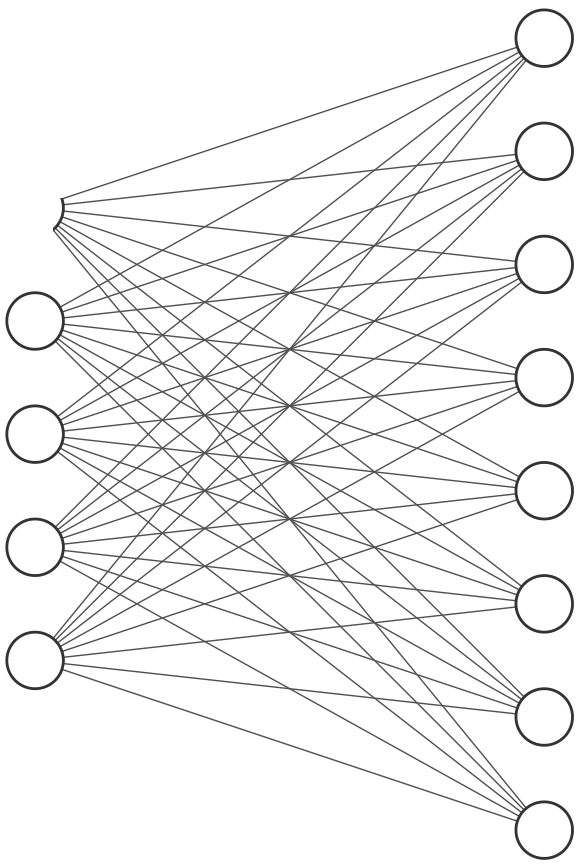
\includegraphics[width=0.5\textwidth]{tu2.png}
%\end{figure}





~\\
\newpage
\noindent\textbf{神经网络张量流:}
\begin{table}[!h]
\resizebox{\textwidth}{!}{
\begin{tabular}{|c|c|c|c|}
\hline
前向传播          & 维度                        & 反向传播                                                 & 维度                                  \\ \hline \hline
X             & $N_T\times (N_t+1)$       & LOSS                                               & Scalar                           \\ \hline
$S^{(1)}$     & $N_T\times N^{(1)}$       & $\Delta^{(H+1)}$                                     & $N_T\times K$                       \\ \hline
$(A^{(1)})^+$     & $N_T\times (N^{(1)}+1)$     & $\nabla_{W^{(H+1)}}\mathcal{L}$   & $(N^{(H)}+1)\times K$           \\ \hline
$S^{(2)}$     & $N_T\times N^{(2)}$       & $\Delta^{(H)}$                                   & $N_T\times (N^{(H)}+1)$         \\ \hline
$(A^{(2)})^+$     & $N_T\times (N^{(2)}+1)$     & $\nabla_{W^{(N)}}\mathcal{L}$ & $(N^{(H-1)}+1)\times N^{(H)}$ \\ \hline
$\vdots$       & $\vdots$                   & $\vdots$                                              & $\vdots$                             \\ \hline
$S^{(H)}$ & $N_T\times N^{(H)}$   & $\Delta^{(i)}$                                       & $N_T\times (N^{(i)}+1)$             \\ \hline
$(A^{(H)})^+$ & $N_T\times (N^{(H)}+1)$ & $\nabla_{W^{(i)}}\mathcal{L}$     & $(N^{(i-1)}+1)\times N^{(i)}$       \\ \hline
$S^{(H+1)}$   & $N_T\times K$             & $\Delta^{(1)}$                                       & $N_T\times (N^{(1)}+1)$             \\ \hline
$A^{(H+1)}$   & $N_T\times K$             & $\nabla_{W^{(1)}}\mathcal{L}$     & $(N_t+1)\times N^{(1)}$             \\ \hline
\multicolumn{2}{|c|}{comput Loss}              & \multicolumn{2}{c|}{update Weight}                   \\ \hline
\end{tabular}}
\end{table}


\paragraph{优化算法}
\subparagraph{批量梯度下降(Batch Gradient Descent,BGD)}

批量梯度下降法是最原始的形式,它是指在每一次迭代时使用所有样本来进行梯度的更新。
\begin{enumerate}
  \item 对目标函数求导:$$\frac{\Delta J\left(\theta_{0}, \theta_{1}\right)}{\Delta \theta_{j}}=\frac{1}{m} \sum_{i=1}^{m}\left(h_{\theta}\left(x^{(i)}\right)-y^{(i)}\right) x_{j}^{(i)}$$

其中 $i=1,2,\cdots,m$ 表示样本数, $j=0,1$ 表示特征数,这里我们使用了偏置项 $x_0^{(i)}=1$ 。
  \item 每次迭代对参数进行更新: $$\theta_{j}:=\theta_{j}-\alpha \frac{1}{m} \sum_{i=1}^{m}\left(h_{\theta}\left(x^{(i)}\right)-y^{(i)}\right) x_{j}^{(i)}$$
\end{enumerate}

\noindent \textbf{伪码:}\\
$\begin{array}{l}{\text { repeat\{ }} \\ {\qquad \begin{array}{l}{\theta_{j}:=\theta_{j}-\alpha \frac{1}{m} \sum_{i=1}^{m}\left(h_{\theta}\left(x^{(i)}\right)-y^{(i)}\right) x_{j}^{(i)}} \\ { \text { (for }j=0,1)} \\ \} \end{array}}\end{array}$


\begin{enumerate}
  \item 优点:
\begin{itemize}
  \item 一次迭代是对所有样本进行计算,此时利用矩阵进行操作,实现了并行。
  \item 由全数据集确定的方向能够更好地代表样本总体,从而更准确地朝向极值所在的方向。当目标函数为凸函数时,BGD一定能够得到全局最优。
\end{itemize}
  \item 缺点:
\begin{itemize}
  \item 当样本数目 m 很大时,每迭代一步都需要对所有样本计算,训练过程很慢。
\end{itemize}
\end{enumerate}

\subparagraph{随机梯度下降(Stochastic Gradient Descent,SGD)}

随机梯度下降法不同于批量梯度下降,随机梯度下降是每次迭代使用一个样本来对参数进行更新。使得训练速度加快。

\begin{enumerate}
  \item 对一个样本的目标函数求偏导:
        $$\frac{\Delta J^{(i)}\left(\theta_{0}, \theta_{1}\right)}{\theta_{j}}=\left(h_{\theta}\left(x^{(i)}\right)-y^{(i)}\right) x_{j}^{(i)}$$
  \item 参数更新:
$$\theta_{j}:=\theta_{j}-\alpha\left(h_{\theta}\left(x^{(i)}\right)-y^{(i)}\right) x_{j}^{(i)}$$
\end{enumerate}

\noindent \textbf{伪码:}\\
$\begin{array}{l}{\text { repeat\{ }}\\ {\qquad \begin{array}{l}{\text{for}~i=1,\cdots,m\{}\\{~~~~~~~~\theta_{j}:=\theta_{j}-\alpha \left(h_{\theta}\left(x^{(i)}\right)-y^{(i)}\right) x_{j}^{(i)}} \\ { ~~~~~~\text { (for }j=0,1)} \\ ~~~~~~~~\} \\ \} \end{array}}\end{array}$

\begin{enumerate}
  \item 优点:
\begin{itemize}
  \item 由于不是在全部训练数据上的损失函数,而是在每轮迭代中,随机优化某一条训练数据上的损失函数,这样每一轮参数的更新速度大大加快。
\end{itemize}
  \item 缺点:
\begin{itemize}
  \item 准确度下降。由于即使在目标函数为强凸函数的情况下,SGD仍旧无法做到线性收敛。
  \item 可能会收敛到局部最优,由于单个样本并不能代表全体样本的趋势。
  \item 不易于并行实现。
\end{itemize}
\end{enumerate}

\subparagraph{小批量梯度下降(Mini-Batch Gradient Descent, MBGD)}

是对 BGD 以及 SGD 的一个折中办法。其思想是:每次迭代 使用 batch\_size 个样本来对参数进行更新。

这里我们假设 batch\_size=10 ,样本数 m=1000 。

\noindent \textbf{伪码:}\\
$\begin{array}{l}{\text { repeat\{ }}\\ {\qquad \begin{array}{l}{\text { for } \mathrm{i}=1,11,21,31, \ldots, 991 \{}\\{~~~~~~~~\theta_{j}:=\theta_{j}-\alpha \frac{1}{10} \sum_{k=i}^{(i+9)}\left(h_{\theta}\left(x^{(k)}\right)-y^{(k)}\right) x_{j}^{(k)}} \\ { ~~~~~~\text { (for }j=0,1)} \\ ~~~~~~~~\} \\ \} \end{array}}\end{array}$


\begin{enumerate}
  \item 优点:
\begin{itemize}
  \item 通过矩阵运算,每次在一个batch上优化神经网络参数并不会比单个数据慢太多。
  \item 每次使用一个batch可以大大减小收敛所需要的迭代次数,同时可以使收敛到的结果更加接近梯度下降的效果。(比如上例中的30W,设置batch\_size=100时,需要迭代3000次,远小于SGD的30W次)
  \item 可实现并行化。
\end{itemize}
  \item 缺点:
\begin{itemize}
  \item batch\_size的不当选择可能会带来一些问题。

\end{itemize}
\end{enumerate}



\newpage
\subsection{MSVL 语言框架}
\textcolor{red}{数据类型 : 单精度浮点数。}

\subsubsection{辅助函数}
\begin{enumerate}
  \item absolute
  \item min
  \item equal
  \item F2S
  \item sigmoid
  \item tanh
  \item relu
  \item leakyRelu
\end{enumerate}



\subsubsection{矩阵操作函数}
\begin{enumerate}
  \item MatCreate
  \item MatDelete
  \item MatSetVal
  \item MatShape
  \item MatDump
  \item MatAdd
  \item MatSub
  \item MatMul
  \item MatProduct
  \item MatNumMul
  \item MatNumAdd
  \item MatTrans
  \item MatZeros
  \item MatOnes
  \item MatEye
  \item MatRowSum
  \item MatRowMax
  \item MatExp
  \item MatSquare
  \item MatVectorSub
  \item MatVectorDiv
  \item MatCopy
  \item MatPlusRow
  \item MatPlusCol
\end{enumerate}



\subsubsection{矩阵激活函数}

\begin{enumerate}
  \item MatNoneActi
  \item MatSoftmax
  \item MatSigmoid
  \item MatTanh
  \item MatRelu
  \item MatLeakyRelu
\end{enumerate}

\subsubsection{矩阵激活函数导数函数}
\begin{enumerate}
  \item MatDerivationNoneActi   0
  \item MatDerivationSigmoid   1
  \item MatDerivationTanh   2
  \item MatDerivationRelu   3
  \item MatDerivationLeakyRelu   4
  \item MatDerivationSoftmax   5
\end{enumerate}

\subsubsection{损失函数}
\begin{enumerate}
  \item OneHot
  \item MSE
  \item CrossEntropy
\end{enumerate}

\subsubsection{损失函数的导函数}
\begin{enumerate}
  \item MSEDerivative
  \item CrossEntropyDerivative
\end{enumerate}

\subsubsection{神经网络的初始化}
\href{https://blog.csdn.net/z_feng12489/article/details/102856968}{神经网络初始化介绍}
\begin{enumerate}
  \item AllZero initialization
  \item Random initialization
  \item \href{https://blog.csdn.net/z_feng12489/article/details/102913634}{Xavier initialization}
  \item He initialization
\end{enumerate}


相关函数
\begin{enumerate}
  \item gaussrand\_NORMAL  标准高斯随机生成
  \item gaussrand 高斯随机生成
  \item MatInitZero 全零初始化
  \item MatInitRandomNormalization 随机初始化
  \item MatInitXavier Xavier初始化
  \item MatInitHe 凯明初始化
\end{enumerate}


\subsubsection{神经网络用户自定义参数}

\begin{table}[!h]
\resizebox{\textwidth}{!}{
\begin{tabular}{|l|l|l|l|}
\hline
用户自定义参数   & 参数表示               & 数据类型    & 备注                                                                                                                                                                                                                                                                                                 \\ \hline\hline
输入训练样本的数量 & N\_sample          & int     & NULL                                                                                                                                                                                                                                                                                               \\ \hline
单一训练样本的维度 & D\_sample          & int     & NULL                                                                                                                                                                                                                                                                                               \\ \hline
训练样本的真值   & Xval               & float * & 数组长度为 N\_sample * D\_sample                                                                                                                                                                                                                                                                        \\ \hline
训练样本的标签   & Yval               & float * & 数组长度为 N\_sample                                                                                                                                                                                                                                                                                    \\ \hline
权值初始化方式   & Style\_initWeight  & int     & \begin{tabular}[c]{@{}l@{}}0  -\textgreater 全0初始化					\\ 1  -\textgreater 随机初始化\\ 2  -\textgreater Xavier初始化\\ 3  -\textgreater 何凯明初始化\end{tabular}                                                                                                                                                \\ \hline
神经网络隐藏层层数 & N\_hidden          & int     & 注意:这里是隐藏层层数。                                                                                                                                                                                                                                                                                       \\ \hline
各层神经元个数   & N\_layerNeuron     & int *   & 数组长度为 0(输入层),1,...,N\_hidden,N\_hidden+1(输出层).                                                                                                                                                                                                                                                     \\ \hline
各层激活函数    & Nstr\_ActiFsHidden & int *   & \begin{tabular}[c]{@{}l@{}}数组长度为 0(输入层),1,...,N\_hidden,N\_hidden+1(输出层).\\ 取值的映射关系:\\ 0  -\textgreater no activation(input layer)\\ 1  -\textgreater sigmoid\\ 2  -\textgreater tanh\\ 3  -\textgreater relu\\ 4  -\textgreater leaky relu\\ 5  -\textgreater softmax (output layer)\end{tabular} \\ \hline
分类类别数     & N\_out             & int     & NULL                                                                                                                                                                                                                                                                                               \\ \hline
输出层损失函数   & Nstr\_LossF        & int     & \begin{tabular}[c]{@{}l@{}}取值映射关系:\\ 0  -\textgreater MSE\\ 1  -\textgreater CE\end{tabular}                                                                                                                                                                                                       \\ \hline
\end{tabular}}
\end{table}


\subsubsection{神经网络的运算所需空间变量及创建所需空间函数}
\begin{table}[!h]
\resizebox{\textwidth}{!}{
\begin{tabular}{|l|l|l|l|}
\hline
神经网络的运算所需空间变量 & 参数表示                 & 数据类型  & 备注                                                                                                                   \\ \hline
神经网络激活值矩阵     & P\_ActiMat           & Mat * & 列表索引i=0(输入层),1,...,N\_hidden,N\_hidden+1(输出层)                                                                        \\ \hline
神经网络激活值矩阵加偏置列 & P\_ActiMatPlus       & Mat * & \begin{tabular}[c]{@{}l@{}}列表索引i=0(输入层),1,...,N\_hidden\\ 加偏置列 偏置列全部置1.输出层不需要Plus\end{tabular}                       \\ \hline
神经网络求和矩阵      & P\_SumMat            & Mat * & \begin{tabular}[c]{@{}l@{}}列表索引i=0(输入层),1,...,N\_hidden,N\_hidden+1(输出层)\\ i=0 时输入层求和矩阵行列置零 无实际含义\end{tabular}       \\ \hline
神经网络权值矩阵      & P\_WeightMat         & Mat * & \begin{tabular}[c]{@{}l@{}}列表索引i=0(输入层),1,...,N\_hidden,N\_hidden+1(输出层)\\ i=0 时输入层求和矩阵行列置零 无实际含义\end{tabular}       \\ \hline
\rowcolor{yellow}神经网络权值偏置矩阵    & P\_WeightBiasMat     & Mat*  & \begin{tabular}[c]{@{}l@{}}列表索引i = 0(输入层), 1, ..., N hidden,N hidden + 1(输出层)\\ i = 0 时输入层求和矩阵行列置零无实际含义\end{tabular} \\ \hline
训练数据标签        & Mat\_oneHot          & Mat   & row=N\_sample col=N\_out                                                                                             \\ \hline
反向传播中间变量矩阵    & P\_DeltaMat          & Mat * & \begin{tabular}[c]{@{}l@{}}列表索引i=0(输入层),1,...,N\_hidden,N\_hidden+1(输出层)\\ i=0 时输入层求和矩阵行列置零 无实际含义\end{tabular}       \\ \hline
权值偏置矩阵导数变量矩阵  & P\_NablaWbMat        & Mat*  & \begin{tabular}[c]{@{}l@{}}列表索引i = 0(输入层), 1, ..., N hidden,N hidden + 1(输出层)\\ i = 0 时输入层求和矩阵行列置零无实际含义\end{tabular} \\ \hline
激活函数对求和值导数矩阵  & P\_ActiFunDerivation & Mat*  & \begin{tabular}[c]{@{}l@{}}列表索引i = 0(输入层), 1, ..., N hidden,N hidden + 1(输出层)\\ i = 0 时输入层求和矩阵行列置零无实际含义\end{tabular} \\ \hline
\end{tabular}}
\end{table}
\newpage
\noindent \textbf{创建所需空间函数:}
\begin{enumerate}
  \item SpaceCreateActi  创建激活值矩阵所需空间
  \item SpaceCreateActiPlus  创建激活值Plus矩阵所需空间
  \item SpaceCreateSum   创建求和值矩阵所需空间
  \item SpaceCreateWeight   创建权值矩阵所需空间
  \item SpaceCreateWeightBias  创建权值偏置矩阵所需空间
  \item SpaceCreateDelta   创建反向传播中间变量矩阵所需空间
\end{enumerate}


\subsubsection{初始化神经网络}
\noindent\textbf{函数:}
\begin{enumerate}
  \item NNinit
\end{enumerate}

\noindent\textbf{说明:}
\begin{enumerate}
  \item 输入数据喂入激活值(plus)矩阵
  \item 标签数据喂入矩阵并且进行独热编码
  \item 选择常用的初始化方式进行权值初始化
\end{enumerate}


\newpage
\subsubsection{神经网络前向传播}
\begin{table}[!h]
\resizebox{\textwidth}{!}{
\begin{tabular}{|l|l|l|l|}
\hline
神经网络向前传播所需参数变量 & 参数表示               & 数据类型  & 备注                                                                                                                                                                                                                                                                                               \\ \hline\hline
神经网络激活值矩阵      & P\_ActiMat         & Mat * & 列表索引i=0(输入层),1,...,N\_hidden,N\_hidden+1(输出层)                                                                                                                                                                                                                                                    \\ \hline
神经网络激活值矩阵加偏置列  & P\_ActiMatPlus     & Mat * & \begin{tabular}[c]{@{}l@{}}列表索引i=0(输入层),1,...,N\_hidden\\ 加偏置列 偏置列全部置1.输出层不需要Plus\end{tabular}                                                                                                                                                                                                   \\ \hline
神经网络求和矩阵       & P\_SumMat          & Mat * & \begin{tabular}[c]{@{}l@{}}列表索引i=0(输入层),1,...,N\_hidden,N\_hidden+1(输出层)\\ i=0 时输入层求和矩阵行列置零 无实际含义\end{tabular}                                                                                                                                                                                   \\ \hline
神经网络权值偏置矩阵     & P\_WeightBiasMat   & Mat * & \begin{tabular}[c]{@{}l@{}}列表索引i = 0(输入层), 1, ..., N hidden,N hidden + 1(输出层)\\ i = 0 时输入层求和矩阵行列置零无实际含义\end{tabular}                                                                                                                                                                             \\ \hline
训练数据标签         & Mat\_oneHot        & Mat   & row=N\_sample col=N\_out                                                                                                                                                                                                                                                                         \\ \hline
神经网络隐藏层层数      & N\_hidden          & int   & 注意:这里是隐藏层层数。                                                                                                                                                                                                                                                                                     \\ \hline
各层激活函数         & NStr\_ActiFsHidden & int * & \begin{tabular}[c]{@{}l@{}}数组长度为 0(输入层),1,...,N hidden,N hidden+1(输出层).\\ 取值的映射关系:\\ 0 -\textgreater{}no activation(input layer)\\ 1 -\textgreater{}sigmoid\\ 2 -\textgreater{}tanh\\ 3 -\textgreater{}relu\\ 4 -\textgreater{}leaky relu\\ 5 -\textgreater{}softmax (output layer)\end{tabular} \\ \hline
输出层损失函数        & Nstr\_LossF        & int   & \begin{tabular}[c]{@{}l@{}}取值映射关系:\\ 0 -\textgreater{}MSE\\ 1 -\textgreater{}CE\end{tabular}                                                                                                                                                                                                     \\ \hline
\end{tabular}}
\end{table}
\begin{enumerate}
  \item MatActivate 激活函数选择函数
  \item LossFunction 损失函数选择函数
  \item NNforward 神经网络前向传播函数-返回损失
\end{enumerate}


\subsubsection{神经网络反向传播}
\begin{table}[!h]
\resizebox{\textwidth}{!}{
\begin{tabular}{|l|l|l|l|}
\hline
神经网络反向传播所需参数变量         & 参数表示                 & 数据类型  & 备注                                                                                                                                                                                                                                                                                               \\ \hline\hline
神经网络隐藏层层数              & N\_hidden            & int   & 注意:这里是隐藏层层数                                                                                                                                                                                                                                                                                      \\ \hline
输入样本的数量                & N\_sample            & int   & 样本数量(训练样本)                                                                                                                                                                                                                                                                                       \\ \hline
各层神经元个数                & N\_layerNeuron       & int * & 数组长度为 0(输入层),1,...,N hidden,N hidden+1(输出层)                                                                                                                                                                                                                                                      \\ \hline
神经网络求和矩阵               & P\_SumMat            & Mat * & 列表索引i=0(输入层),1,...,N\_hidden,N\_hidden+1(输出层)                                                                                                                                                                                                                                                    \\ \hline
i=0 时输入层求和矩阵行列置零 无实际含义 & P\_ActiMat           & Mat * & 列表索引i=0(输入层),1,...,N\_hidden,N\_hidden+1(输出层)                                                                                                                                                                                                                                                    \\ \hline
神经网络激活值矩阵加偏置列          & P\_ActiMatPlus       & Mat * & \begin{tabular}[c]{@{}l@{}}列表索引i=0(输入层),1,...,N\_hidden\\ 加偏置列 偏置列全部置1.输出层不需要Plus\end{tabular}                                                                                                                                                                                                   \\ \hline
反向传播中间变量矩阵             & P\_DeltaMat          & Mat * & \begin{tabular}[c]{@{}l@{}}列表索引i = 0(输入层), 1, ..., N hidden,N hidden + 1(输出层)\\ i = 0 时输入层求和矩阵行列置零无实际含义\end{tabular}                                                                                                                                                                             \\ \hline
训练数据标签                 & Mat\_oneHot          & Mat   & row = N\_sample col = N\_out                                                                                                                                                                                                                                                                     \\ \hline
训练数据标签                 & Mat\_oneHot          & Mat   & row=N\_sample col=N\_out                                                                                                                                                                                                                                                                         \\ \hline
各层激活函数                 & NStr\_ActiFsHidden   & int * & \begin{tabular}[c]{@{}l@{}}数组长度为 0(输入层),1,...,N hidden,N hidden+1(输出层).\\ 取值的映射关系:\\ 0 -\textgreater{}no activation(input layer)\\ 1 -\textgreater{}sigmoid\\ 2 -\textgreater{}tanh\\ 3 -\textgreater{}relu\\ 4 -\textgreater{}leaky relu\\ 5 -\textgreater{}softmax (output layer)\end{tabular} \\ \hline
输出层损失函数                & Nstr\_LossF          & int   & \begin{tabular}[c]{@{}l@{}}取值映射关系:\\ 0 -\textgreater{}MSE\\ 1 -\textgreater{}CE\end{tabular}                                                                                                                                                                                                     \\ \hline
激活函数对求和值导数矩阵           & P\_ActiFunDerivation & Mat * & \begin{tabular}[c]{@{}l@{}}列表索引i = 0(输入层), 1, ..., N hidden,N hidden + 1(输出层)\\ i = 0 时输入层求和矩阵行列置零无实际含义\end{tabular}                                                                                                                                                                             \\ \hline
\end{tabular}}
\end{table}

\begin{enumerate}
  \item ActiFunDerivation
  \item LossFunDerivation
  \item NNOuputLayerBackward
  \item NNBackward
\end{enumerate}

\subsubsection{优化算法}

\begin{enumerate}
  \item BGD(批量梯度下降)
  \item SGD(随机梯度下降)
  \item MBGD(小批量梯度下降)
  \item Adam
\end{enumerate}

\textcolor{red}{demo 成型,损失减小,可收敛。}


\newpage
\subsection{MSVL 语言框架重构}
\subsubsection{对象结构体}

\begin{enumerate}
  \item 矩阵~结构体
\begin{lstlisting} [language=c]
typedef struct {
	int row, col;      // rowNum and columnNum [int]
	float** element;   // element, two dimensions
}Mat;
\end{lstlisting}
  \item BP单层~结构体
\begin{lstlisting} [language=c]
typedef struct{
	Mat ActiMat;               // active value Matrix without bias column
	Mat ActiMatPlus;           // active value Matrix with bias column
	Mat SumMat;                // sum value Matrix
	Mat WeightMat;             // weight value Matrix without bias row
	Mat WeightBiasMat;         // weight value Matrix with bias row
	Mat DeltaMat;              // backtrack temporary variable Matrix
	Mat NablaWbMat;            // gradient Matrix for weight with bias
	Mat ActiFunDerivationMat;  // active Function Dervation Matrix

	int NeuronNum;             // number of neuron [int]
	int AcitFuncNum;           // active function [int]
}FCLayer;
\end{lstlisting}
  \item BP神经网络~结构体
\begin{lstlisting} [language=c]
typedef struct{
	int CurrentSampleNum;             // number of current samples [int]
	int SampleDimensionNum;    // dimensions(features) of sample [int]
	int HiddenLayerNum;        // number of hidden layer [int]
	int WeightInitWayNum;      // weight initialization mode [int]

	FCLayer *Layer;            // layers of FCNN
	Mat OnehotMat;             // onehot code Matrix

	int ClassificationNum;     // Number of categories classified [int]
	int LossFuncNum;           // loss function [int]
}FCNN;
\end{lstlisting}
  \item 用户自定义参数~结构体
\begin{lstlisting} [language=c]
typedef struct{
    int CompleteSampleNum;		// number of all samples [int]
	int TrainSampleNum;			// number of training samples [int]
	int TestSampleNum;			// number of test samples [int]
	int ValidationNum;			// number of validation samples [int]
	int SampleDimensionNum;    // dimensions(features) of sample [int]
	int HiddenLayerNum;        // number of hidden layer [int]
	int WeightInitWayNum;      // weight initialization mode [int]
	float *XValArray;          // samples features value [float*]
	float *YValArray;          // samples labels value [float*]
	int *NeuronNumArray;       // numbers of every layers Neuron [int*]
	int *ActiFuncNumArray;     // activate functions of every layers [int*]
	int ClassificationNum;     // Number of categories classified [int]
	int LossFuncNum;           // loss function [int]
}Custom;
\end{lstlisting}
%   int OptiAlgNum;            // optimize algorithm [int]
%   float lr;                  // learning rate for optimize algorithm[float]
%   int batch;                 // batch number for optimize algorithm [int]

\item 数据集~结构体
\begin{lstlisting} [language=c]
typedef struct{
	Mat CompleteFeatureDataSet;	// complete featrue Mat for FCNN
	Mat CompleteLabelDataSet;	// complete label Mat without onehot
	Mat CompleteTrainFeature;	// complete featrue Mat for FCNN training
	Mat CompleteTrainLabel;		// complete label Mat without onehot
	Mat *BatchTrainFeature;		// batch featrue Mat for FCNN training [three dimensions]
	Mat *BatchTrainLabel;		// batch label Mat without onehot [three dimensions]
	Mat *BatchTrainLabelOneHot; // batch label Mat with onehot [three dimensions]
	Mat TestFeature;			// featrue Mat for FCNN test
	Mat TestLabel;				// label Mat without onehot
	Mat TestLabelOneHot;        // label Mat with onehot
	//Mat ValidationFeature;	// featrue Mat for FCNN Validation
	//Mat ValidationLabel;		// label Mat withoutone
	

	int CompleteSampleNum;		// number of all samples [int]
	int TrainSampleNum;			// number of training samples [int]
	int TestSampleNum;			// number of test samples [int]
	//int ValidationNum;			// number of validation samples [int]
	int SampleDimensionNum;    // dimensions(features) of sample [int]
	int ClassificationNum;     // Number of categories classified [int]
	int BatchSize;				// batch size for dataset
	int BatchNum;				// number of batch
	int remainder;				// the last batch size
}DataSet;
\end{lstlisting}
\end{enumerate}




\textcolor{red}{\fbox{batch} 机制的实现:建立 \fbox{batch} 结构体,分割数据集,复制到  \fbox{FCNN}  中。}

其中 $\text{TrainSampleNum} = \text{BatchSize}*\text{BatchNum}+\text{remainder}$,当$\text{remainder}=0$时,代表能被整除。

\subsubsection{开发流程}
\begin{enumerate}
  \item 用户自定义参数及总数据录入;
  \item 数据集构建;
  \item 神经网络初始化;
  \item 前向传播构建;
  \item 反向传播构建;
  \item 优化算法构建;
  \item 神经网络训练构建;
  \item 神经网络测试构建。
\end{enumerate}


\paragraph{神经网络用户自定义参数及总数据录入}~目的是将相关参数及总的数据赋值给用户自定义结构体中(其中注意对数组数据的赋值,传引用即可),再将各个参数分发给各个结构体。


\paragraph{数据集构建} ~根据用户输入的数据相关参数将训练测试数据集构建完成。构建路线:
\begin{enumerate}
  \item 根据训练集数据量以及 $\text{Batch\_Size}$ 大小计算并导入相关参数。
  \item 根据整体数据集的各个参数,开辟所需的全部空间。
  \item 将整体数据集数组根据训练测试集数目划分成两个数组,包括训练特征数组和训练标签数组,测试特征数组和测试标签数组。
  \item 再将训练特征数组和训练标签数组划分成若干个块大小的块训练特征数组和块训练标签数组。
  \item 最后将数据喂入到相应的矩阵结构体当中。
\end{enumerate}


\paragraph{神经网络初始化}
\begin{enumerate}
  \item 开辟神经网络所需空间并导入每层相关参数\textcolor{red}{注意创建顺序不可变化。}
  \begin{enumerate}[(1)]
    \item 创建神经网络层空间
    \begin{enumerate}[<1>]
      \item FCLayer
    \end{enumerate}
        \item 导入每层参数
    \begin{enumerate}[<1>]
      \item NeuronNum
      \item AcitFuncNum
    \end{enumerate}
    \item 创建神经网络运算空间
    \begin{enumerate}[<1>]
      \item ActiMat
      \item ActiMatPlus
      \item SumMat
      \item ActiFunDerivationMat
      \item DeltaMat
      \item OnehotMat(FCNN)
    \end{enumerate}
    \item 创建神经网络参数空间\textcolor{red}{(参数空间的大小不随输入神经网络样本大小而改变)}
    \begin{enumerate}[<1>]
      \item WeightMat
      \item WeightBiasMat
      \item NablaWbMat
    \end{enumerate}
  \end{enumerate}
  \item 进行权值初始化
  \begin{enumerate}
    \item WeightMat
    \item WeightBiasMat
  \end{enumerate}
\end{enumerate}



\paragraph{神经网络前向传播求损失} ~神经网络向前传播将小批量输入样本导入神经网络输入层激活值矩阵,并将对应的标签数据进行独热编码,然后进行矩阵运算损失处理得到标量损失值。\textcolor{red}{其中要注意小批量输入样本的数量不一定和已经开辟的神经网络有关矩阵空间的数量相一致,要做检查处理。}

\begin{enumerate}
  \item 小批量余数处理
  \item 输入特征数据拷贝到激活值矩阵
  \item 输入标签独热编码数据拷贝到神经网络独热编码矩阵中
  \item 前向传播矩阵相乘,激活,扩展激活值矩阵
  \item 预测值矩阵与真实值矩阵求损失,返回
\end{enumerate}

\paragraph{神经网络反向传播求梯度} ~神经网络先经过一次正向传播得到损失之后,再求其损失对所有权值偏置的导数得到梯度,用到了\textcolor{red}{反向传播算法}。注意,每一次反向传播是建立在一次正向传播求得损失的基础之上的。

\begin{enumerate}
  \item 输出层反向传播,求得输出层的中间变量矩阵以及权值导数
  \item 隐藏层反向传播,求得各隐藏层的中间变量矩阵以及权值导数
\end{enumerate}

\paragraph{Adam算法构建}~Adam算法使用了\textcolor{red}{动量变量$~v_t~$}和\textcolor{red}{RMSProp算法中小批量随机梯度按元素平方的指数加权移动平均变量$~s_t~$},并在时间步0将它们中每个元素初始化为0。\\
默认参数变量:$\beta_1=0.9, \beta_2=0.999, \eta=10^{-3}, \epsilon=10^{-8}$。
\begin{align}
  & v_t=\beta_1v_{t-1}+(1-\beta_1)g_t\\
  & s_t = \beta_2s_{t-1}+(1-\beta_2)g_t\odot g_t \\
  & \hat{v}_t=\frac{v_t}{1-\beta^t_1}\\
  & \hat{s}_t=\frac{s_t}{1-\beta^t_2}\\
  & g'_t=\frac{\eta \hat{v}_t}{\sqrt{\hat{s}_t}+\epsilon}\\
  & x_t = x_{t-1}- g'_t
\end{align}
\begin{enumerate}
  \item 创建Adam参数结构体。
  \item 初始化结构体参数。
  \begin{enumerate}
    \item 初始化参变量为默认值。
    \item 创建变量所需空间。
    \item 时间步设置为0。
  \end{enumerate}
  \item 根据六个公式更新梯度。
\end{enumerate}

\newpage
\subsection{FCNN应用}
\subsubsection{Minst 手写字体识别}

\begin{enumerate}
  \item 数据集构建。\\
  minst 手写字体识别数据集包括一共 70000 张灰度图片,每张图片 28$\times$28 个像素,图片数据集包括 0$\sim$9 十类。全体数据集是经过出最大值归一化后的数据集。
  \item 神经网络搭建。
\begin{lstlisting}
CompleteSampleNum:	70000
TrainSampleNum:		60000
TestSampleNum:		10000
SampleDimensionNum:	784
HiddenLayerNum:		2
WeightInitWayNum:	3
ClassificationNum:	10
LossFuncNum:		1
BatchSize:		100
XValArray:(length = 54880000)	
YValArray:(length = 70000)	
NeuronNumArray:	
784	512	256	10	
ActiFuncNumArray:(include output layer Acti-Function)	
0	3	3	5	
OptimizationMethod: Mini-Batch Stochastic gradient descent
  \end{lstlisting}
\end{enumerate}

\begin{enumerate}
  \item BSGD 收敛性不佳,指的是时间以及准确度上都达不到要求;
  \item 开发Adam优化算法,提高准确度提高了五个百分点,以及收敛时间都缩短了1.5倍。
  \item 对稀疏矩阵的运算做优化,收敛时间有缩短了一倍。
\end{enumerate}

\newpage
\part{开题报告}

\section{题目}
基于MSVL的神经网络基础建模框架的设计与实现

Design and Implementation of Fundamental Modeling Framework for Neural Networks based on MSVL


\section{论文概况}
\subsection{选题来源}
国家自然科学基金项目

\subsection{摘要}

本文对神经网络的形式化建模方法进行研究,旨在为神经网络系统进行形式化验证提供模型理论基础。随着人工智能和神经网络的不断发展以及在计算机视觉,数据处理等领域的广泛应用,如何保障神经网络系统安全可靠成为了一个迫切需要解决的问题。目前,国内外关于神经网络系统安全性的研究集中在攻防方法的开发上,较少有工作使用形式化的手段对这类系统的安全性予以验证。本文以建模仿真语言MSVL以及投影时序逻辑PTL为基础,拟对神经网络的张量运算,初始化,激活函数,损失函数,优化方法等基本操作或者构件进行形式化建模研究,开发一套神经网络的基础建模框架,为CNN,RNN等其他类型的深度学习模型的形式化建模提供理论基础,为神经网络的形式化验证提供建模基础。

\section{选题依据}

\subsection{选题意义}

在如今飞速发展的机器学习和人工智能领域中,神经网络已经占据了重要地位。借助于卷积神经网络、循环神经网络等神经网络模型以及深度学习技术,神经网络系统拥有了出色的数据运算和类别预测能力。
这类系统已成功应用于计算机视觉、自然语言处理、数据挖掘等领域,具备图像分类、语音识别、数据分析、智能推荐等丰富而方便的功能。其中不乏人们所熟知的系统,如人脸识别系统、自动驾驶汽车控制系统、阿尔法围棋等。

然而,即便神经网络系统已经展示了在处理复杂问题时所取得的成功,但是它们也有其严重的安全漏洞。对于图像系统来说,具有较小扰动的对抗性样本不能为人所察觉,但是它们可以轻而易举地愚弄了神经网络模型。这种对抗攻击对神经网络系统造成了一系列威胁,也促使了这个方向上的大量研究投入。谷歌大脑也有研究表明,任何机器学习分类器都可能被欺骗,给出不正确的预测。在自动语音识别(ASR)系统中,深度循环网络已经取得了一定的成功,但是许多人已经证明,小的对抗干扰同样可以欺骗深层神经网络。

具体来说,在2016年6月,美国特斯拉公司的一辆 Model-S 型电动轿车在自动驾驶模式下撞上了一辆大型牵挂型卡车,导致一人当场身亡。事故原因是自动驾驶系统未能识别出前方卡车的白色侧面,以致没有及时启动刹车。2017年 11月的一个晚上,德国警方闯入一间公寓,因为他们接到邻居的报警,抱怨大清早就被隔壁震耳欲聋的音乐吵醒,然而这不是一个聚会,而是亚马逊的 Echo 在主人外出时,随机播放了音乐。2018年3月18日,一辆Uber自动驾驶车辆在美国亚利桑那州与一名行人相撞并致其死亡,成为全球首例自动驾驶致行人死亡事故。

值得指出的是,神经网络系统的形式化建模与验证并不是一个简单的问题。据我们了解,目前这一方面的研究工作也有限。究其原因,神经网络系统的运行依赖于由机器学习而得到的参数,其行为尚不透明、不可解释。如何为这类系统建立形式化模型以及如何对系统的安全性质进行形式化定义都是不小的挑战。此外,神经网络系统与大数据密切相关,系统的训练样本集和内部参数往往规模庞大,这无疑增加了验证的难度。神经网络系统的形式化建模与验证是一个迫切需要研究的问题,而这一问题的基础在于为神经网络建立形式化模型。

\subsection{国内外研究现状}

近年来,随着神经网络系统大规模的开发和应用,它们的安全性受到了研究人员越来越多的关注。由此开展了众多关于神经网络系统所面临的安全威胁及相应的防御技术的研究。

Szegedy 等人首次证明了可以通过对图像添加小量的人类察觉不到的扰动误导神经网络做出误分类。他们首先尝试求解让神经网络做出误分类的最小扰动的方程。但由于问题的复杂度太高,他们转而求解简化后的问题,即寻找最小的损失函数添加项,使得神经网络做出误分类,这就将问题转化成了凸优化过程。Ian J.Goodfellow 等人利用符号函数有目的地在图像样本上施加微小的扰动,提出了一种快速产生对抗样本的方法,并以高可信度在手写识别数据集上得到了验证。Moosavi-Dezfooli 等人通过迭代计算的方法生成最小规范对抗扰动,将位于分类边界内的图像逐步推到边界外,直到出现错误分类,结果证明他们生成的扰动比 FGSM 更小,同时有相似的欺骗率等。除了在神经网络系统分类任务攻击以外,还可以对自编码器和生成模型,循环神经网络,深度强化学习,语义分割和物体检测上进行攻击,攻击效果也非常可观。而在这种对抗攻击上的防御策略也主要存在三个方向,修改训练过程或者样本;修改网络;附加网络。但都未利用到形式化的手段。

近些年来,有为数不多的利用形式化手段对神经网络的攻击与防御进行验证的工作。Huang 等人通过定义一组操纵对标准样本的邻域空间离散化,由此建立一组逻辑约束,并使用可满足模理论(SMT)求解器检验标准样本邻域空间中是否存在对抗样本。同样采用 SMT 求解技术,Scheibler 等人验证了倒立摆控制系统的特定性质,如状态的可达性。然而,其神经网络规模较小,仅包含 4 层共 16 个神经元。Katz 等人提出了一种针对仅采用修正线性单元(ReLU)激活函数的深度神经网络的验证方法。该方法通
过对线性规划的单纯形法进行扩展,使其支持 ReLU 函数,进而对这类神经网络的线性性质加以验证。此外,Ghodsi 等人提出了一种对部署在云端的神经网络
系统的验证方法。该方法对神经网络的结构做出了一些限制,如数据在有穷域内、仅采用二次激活函数等,通过一定的交互式证明协议验证系统的正确性。%【基础简化的神经网络数学模型,某种限制的神经网络数学模型】

目前为止,对于神经网络的验证都是基于神经网络的朴素的数学模型,并且仅考虑了模型中特定的方面,做了特定的简化假设,进而验证特定的性质。据本人所知,目前还没有工作采用一种形式化语言对神经网络的整体进行建模。本工作正是针对现状的这一不足旨在利用MSVL这种形式化语言,对神经网络的结构、行为(包括训练和预测)进行综合性建模。为进一步验证神经网络的性质提供基础。


%目前对于神经网络系统的攻击方法大多都是基于神经网络的数值特征进行的,而常见的主被动防御措施的防御效果又很难得到保证,而利用形式化方法对神经网络系统的攻击与防御的研究又为数不多,而神经网咯的形式化建模研究更是寥寥无几。在此背景下,利用研究所开发的一种由投影时序逻辑(PTL)所定义的形式化语言:建模、仿真和验证语言(MSVL)为神经网络系统进行建模,为验证神经网络系统性质,研究神经网络系统攻防技术提供基础。



\section{研究方案}

\subsection{研究目标}
对神经网络的形式化建模进行研究,形成基础的神经网络建模理论方法,支持对神经网络的训练、测试进行综合性建模。开发BP神经网络的建模工具,该工具可由用户自定义神经网络参数,生成神经网络的综合性形式化模型。

\subsection{研究内容}
为实现上述研究目标,本文基于形式化语言MSVL,研究神经网络各要素的建模方法,具体包括以下几点。
\begin{enumerate}[(1)]
  \item 对逻辑,算数和矩阵运算进行形式化建模。
  \item 对神经网络的几种权值初始化方式进行形式化建模。
  \item 对神经网络的几种激活函数进行形式化建模。
  \item 对神经网络的几种损失函数进行形式化建模。
  \item 对神经网络的前项传播进行形式化建模。
  \item 对神经网络的反项传播进行形式化建模。
  \item 对基于梯度的优化方法进行形式化建模。
\end{enumerate}

\subsection{拟解决关键问题}
\begin{enumerate}[(1)]
  \item 如何利用基于时序逻辑的语言MSVL对神经网络进行形式化建模。
  \item 如何建立综合性的、可扩展的神经网络形式化模型。
\end{enumerate}

\subsection{拟采取的研究方法、技术路线、实验方案及可行性研究}
\begin{enumerate}[(1)]
  \item 研究方法:\\
  $\text{\quad\quad}$实验研究,对现有的理论进行创新、完善或扩充,理论扩展其应用范围,并完成
相应的模块单元测试,实现具体的模块功能。
  \item 技术路线:\\
\begin{figure}[!h]
  \centering
  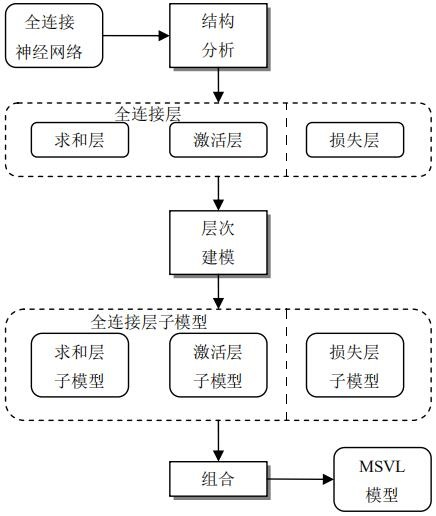
\includegraphics[width=0.5\textwidth]{FCNN.jpg}
\end{figure}

$\text{\quad\quad}$关于形式化模型的选择,拟采用基于 MSVL 语言的模型。一方面,MSVL 语言由投影时序逻辑 PTL 所定义,具备严格的逻辑基础。另一方面,该语言支持多种基本类型与复合类型,函数、框架等重要机制以及顺序、并发、选择、循环等多种控制结构,适用于此系统的建模。

$\text{\quad\quad}$神经网络系统的形式化建模从系统的结构出发,逐层开展,完整的系统模型
由各层次的模型组合而得。其核心步骤是包括数据结构和运算行为进行建模。之后的技术路线:

%\noindent \textbf{变量说明:}
%
%\begin{table}[!h]
%\resizebox{\textwidth}{!}{
%\begin{tabular}{|l|l|l|}
%\hline
%变量          & 含义           & 备注                                                                                                                           \\ \hline
%$X$           & 输入训练样本       & 维度 $N_T\times N_t$,相当于激活值矩阵$A^{(0)}$.                                                                        \\ \hline
%$X^+$           & 输入训练样本加偏置列       & 维度 $N_T\times (N_t+1)$,相当于激活值矩阵$\big(A^{(0)}\big)^+$.                                                                        \\ \hline
%$S^{(i)}$   & 第 i 层求和值矩阵 & 维度 $N_T\times N^{(i)}$, $i=1,\cdots,N,N+1$.                                                                                \\ \hline
%$A^{(i)}$   & 第 i 层激活值矩阵 & 维度 $N_T\times N^{(i)}$, $i=0,1,\cdots,N,N+1$.                                                                              \\ \hline
%$\big(A^{(i)}\big)^+$   & 第 i 层激活值矩阵加偏置列 & 维度 $N_T\times (N^{(i)}+1)$, $i=0,1,\cdots,N$.                                                                              \\ \hline
%$W^{(i)}$   & 第 i 层权值矩阵  & 维度 $N^{(i-1)}\times N^{(i)}$, $i=1,\cdots,N,N+1$.                                                                                                  \\ \hline
%$W^{(N+1)}$ & 输出层权值矩阵      & 维度 $N^{(N)}\times K$, 标签有 K 个类目。                                                                                     \\ \hline
%$W_b^{(i)}$   & 第 i 层权值偏置矩阵  & 维度 $(N^{(i-1)}+1)\times N^{(i)}$, $i=1,\cdots,N,N+1$.                                                                                                  \\ \hline
%$W_b^{(N+1)}$   &输出层权值偏置矩阵  & 维度 $(N^{(N)}+1)\times K$, 标签有 K 个类目。                                                                                                 \\ \hline
%$S^{(N+1)}$ & 输出层求和值矩阵     & 维度 $N_T\times K $.                                                                                                           \\ \hline
%$A^{(N+1)}$ & 输出层激活值矩阵     & 维度 $N_T\times K $.                                                                                                           \\ \hline
%$Y$ & 训练数据标签 & 维度 $N_T \times K$ (ONE-HOT).\\ \hline
%$\Delta^{(i)}$ & 第 i 层的反向传播中间变量矩阵 & 维度 $N_T \times N^{(i)}$, $i=1,\cdots,N,N+1$.\\ \hline
%$\Delta^{(N+1)}$ & 输出层反向传播中间变量矩阵 & 维度 $N_T \times K$.\\ \hline
%\end{tabular}}
%\end{table}


  \begin{enumerate}[(a)]
    \item 神经网络的前向传播进行建模。
 %   \begin{align*}
%   \big(A^{(0)}\big)^+W_b^{(1)}=S^{(1)}\stackrel{\sigma+b}{\longrightarrow} \big(A^{(1)}\big)^+&\Rightarrow \cdots \Rightarrow \cdots \\
%  & \Rightarrow \big(A^{(N-1)}\big)^+W_b^{(N)}=S^{(N)} \stackrel{\sigma+b}{\longrightarrow}\big(A^{(N)}\big)^+  \\
%  & \Rightarrow \big(A^{(N)}\big)^+W_b^{(N+1)}=S^{(N+1)}\stackrel{\sigma}{\longrightarrow} A^{(N+1)} \\
%  & \Rightarrow ~\mathcal{L}(A^{(N+1)},Y)
%\end{align*}
    \item 神经网络的反向传播进行建模。
%    \begin{enumerate}
%  \item 输出层权值求导:
%  \begin{align*}
%  \nabla_{W_b^{(N+1)}}\mathcal{L}(A^{(N+1)},Y) &= \frac{1}{N_T}(A^{(N)^+})^T\Delta^{(N+1)}~~~~~~\text{(矩阵化)}\\
%  \Delta^{(N+1)}& = \frac{\partial \mathcal{L}(A^{(N+1)}, Y)}{\partial A^{(N+1)}}\circ\sigma'(S^{(N+1)})\\
%  \text{当输出层使用 Soft}&\text{max+CrossEntropy 时:}\\
%  \Delta^{(N+1)} &= A^{(N+1)} - Y
%\end{align*}
%  \item 隐藏层权值求导:
%\begin{align*}
%  \nabla_{W_b^{(N)}}\mathcal{L}(A^{(N+1)},Y)&= \frac{1}{N_T}\big(A^{(N-1)^+}\big)^T\Delta^{(N)}\\
%                                \text{令:}       \Delta^{(N)} &=  \big(\Delta^{(N+1)}(W^{(N+1)})^T\big)\circ \sigma'^{(N)}(S^{(N)})\\
%    \text{\textcolor{red}{\sffamily扩展:~对于第 i 个隐藏层}}&\text{\textcolor{red}{\sffamily的权值矩阵的梯度为($i=1,2,\cdots,N.$):}}\\
%    \nabla_{W_b^{(i)}}\mathcal{L}(A^{(N+1)},Y)&= \frac{1}{N_T}\big(A^{(i-1)^+}\big)^T\Delta^{(i)}\\
%                                \text{令:}       \Delta^{(i)} &=  \Delta^{(i+1)}(W^{(i+1)})^T\circ\sigma'^{(i)}(S^{(i)})
%\end{align*}
%\end{enumerate}
    \item 对优化算法进行建模。
 %   \noindent \textbf{伪码:}\\
%$\begin{array}{l}{\text { repeat\{ }}\\ {\qquad \begin{array}{l}{\text { for } \mathrm{i}=1,11,21,31, \ldots, 991 \{}\\{~~~~~~~~\theta_{j}:=\theta_{j}-\alpha \frac{1}{10} \sum_{k=i}^{(i+9)}\left(h_{\theta}\left(x^{(k)}\right)-y^{(k)}\right) x_{j}^{(k)}} \\ { ~~~~~~\text { (for }j=0,1)} \\ ~~~~~~~~\} \\ \} \end{array}}\end{array}$
  \end{enumerate}

  \qquad例如,对于矩阵以及一个单层的神经网络课建模为如下形式化结构:
  \begin{lstlisting} [language=c]
typedef struct {
	int row, col;      // rowNum and columnNum [int]
	float** element;   // element, two dimensions
}Mat;
\end{lstlisting}
\begin{lstlisting} [language=c]
typedef struct{
	Mat ActiMat;               // active value Matrix without bias column
	Mat ActiMatPlus;           // active value Matrix with bias column
	Mat SumMat;                // sum value Matrix
	Mat WeightMat;             // weight value Matrix without bias row
	Mat WeightBiasMat;         // weight value Matrix with bias row
	Mat DeltaMat;              // backtrack temporary variable Matrix
	Mat NablaWbMat;            // gradient Matrix for weight with bias
	Mat ActiFunDerivationMat;  // active Function Dervation Matrix

	int NeuronNum;             // number of neuron [int]
	int AcitFuncNum;           // active function [int]
}FCLayer;
\end{lstlisting}
  \item 实验方案:
  \begin{enumerate}
    \item 查阅相关文献,学习投影时序逻辑的相关理论;
    \item 查阅文献和观看视频资料,学习经典神经网络的结构和建模细节;
    \item 利用MSVL进行神经网络模型搭建。
  \end{enumerate}
  \item 可行性分析:
  \begin{enumerate}
    \item 论文《MSVL a Typed Language for Temporal Logic Programming》使用逻辑定义了一种编程语言,对常用的数据类型,顺序,条件,循环结构等进行了严格的逻辑定义,并开发了一套程序语言MSVL。
    \item 论文《Full Regular Temporal Property Verification as Dynamic Pro\-gram Execution》提出了一种程序可动态执行统一模型检测方法,同 时开发了统一模型检测器 UMC4MSVL;
    \item 论文《A compiler for MSVL and its applications》基于 LLVM 完成一
个名为 MC 的编译器服务于建模仿真验证语言 MSVL,同时分析了 MC 应用
于人工智能 AI 的可行性。
  \end{enumerate}
\end{enumerate}


\subsection{研究计划及预期取得的研究成果}
\begin{table}[!h]
\resizebox{\textwidth}{!}{
\begin{tabular}{|l|l|}
\hline
时间节点            & 预期研究成果                                     \\ \hline
2020.03-2020.05   & 查阅相关文献,完成基本的调研任务,包括对 PTL 词法语法的理解;          \\ \hline
2020.05-2020.06   & 研究 MC 编译器相关的内容,了解 MSVL 相关的编程技术;            \\ \hline
2020.06-2020.08   & 研究经典深度神经网络的结构和训练细节;                        \\ \hline
2020.08-2020.10  & 完成逻辑运算,算数运算,矩阵运算的原型系统建模工作,分析并测试相关性质;       \\ \hline
2020.10-2020.12 & 完成神经网络的初始化,几种损失函数,激活函数的建模工作,分析并测试相关性质;     \\ \hline
2021.12-2021.03  & 完成神经网络的前向传播,梯度优化方式,反向传播的建模工作,并分析测试相关性质;    \\ \hline
2021.03-2021.04   & 完善整体设计的流程,改善系统框架的结构,测试并验证最终的BP神经网络工具的分类回归性能; \\ \hline
2021.04-2021.05   & 撰写论文。                                      \\ \hline
\end{tabular}}
\end{table}


\section{研究基础}
\subsection{已具备的实验条件和研究工作积累}
\begin{enumerate}
  \item 研究条件:电脑、MC 编译器、C2MSVL 转换器、UMC4MSVL 验证器。
  \item 研究工作积累:实验室具有一套完整的 PTL 模型理论,通过学习,对投影
时序逻辑有了一定的认知,并且通过查阅深度神经网络技术相关的论文,有了比较成熟的设计思路。
\end{enumerate}

\subsection{已取得的科研成果    }
无。


\end{CJK}

\end{document}   